\chapter{Density functional theory as a screening method for dense metal membranes}

\section{Abstract}
In this chapter 18 different palladium based membrane materials were simulated in order to determine their suitability as a material for hydrogen impurity enrichment. The alloys were represented using $2\times 2\times 5$ atomic slab models comprised of palladium, with varying compositions of different metals including common palladium additives (Au, Ag, Cu), and metals known for their resistance against aggresive environments (Zr, Cu). From the alloy compositions tested 16/18 were stable, with Cr containing alloys unable to form a stable system. The 16 remaining alloys were then tested with hydrogen, and each of the ISO 14687-2 impurities adsorbed on the 4 avaliable surface sites for hydrogen adsorption. The results were that the impurities could be split into four broad groups. Inert impurities included NH\textsubscript{3}, CO\textsubscript{2}, N\textsubscript{2}, He, Ar and formic acid, which did not interact with the surface of the alloys. Oxidising impurities included H\textsubscript{2}O and O\textsubscript{2}, which pure palladium alone was completely resistant against. The effect could be amplified through the addition of Au and Ag, with PdAu\textsubscript{20} being the best performing alloy for resisting these impurities. Carbonaceous impurities included CO and CH\textsubscript{4} where PdAu\textsubscript{20} was again the best performing alloy, with an average binding energy of CO and CH\textsubscript{4} of around $\times 0.4$ and $\times 0.5$ compared to binding of H. Finally sulphorous atmospheres were tested using H\textsubscript{2}S where PdCuZr and PdAuZr alloys were the best performing. These alloys showed an average binding energy of $\times 0.52$ and $\times 0.49$ compared to H. Formaldehyde was a special case where no alloy composition was found to resist binding. 

This study shows that DFT can be used to give an indication on the suitability of a palladium alloy membrane for it's desired purpose. It also shows that while the effects of some impurities on the surface of a palladium alloy membrane can be completely mitigated, many cannot be inhibited completely. A number of alloys were identified as the best options for hydrogen impurity detection and will be studied experimentally in the following chapters.

\section{Introduction}
Metal membranes operate by selectively dissociating hydrogen, which then allows the hydrogen atoms to subsequently permeate through the bulk of the separation layer. The problem in using palladium membranes as a material for performing hydrogen impurity enrichment is that many hydrogen impurities are also capable of adsorbing onto, and interacting with palladium membranes. The impact of this adsorption can vary depending the molecule, Carbon monoxide for example will simply adsorb onto the surface and result in competitive adsorption between the hydrogen and impurity. Sulphur containing impurities present more of a problem since they can potentially react with many metals used for hydrogen separation membranes. The impact of these contaminants can be minimized by designing alloy compositions that have a weaker attraction to the membrane, and therefore will have less of an affect at higher temperatures where these membranes operate.

Physically testing each potential membrane composition would be time consuming and costly due to the high price of palladium, the time required to synthesise specific membrane compositions, and performing the tests. Simulations provide a solution to this, allowing potential alloys to be quickly screened for their interaction strength with each individual ISO 14687-2 impurity, avoiding the costly and time consuming process of manufacturing each alloy composition. 

In this chapter, 18 dense metal alloy membranes will be simulated using DFT density functional theory as described in section \ref{exp-DFTparams} \cite{QE-2009, QE-2017, doi:10.1063/5.0005082}. The metals will first be evaluated in terms their ability to form a stable alloy, with low risk of segregation, or failure. All stable metals will then be simulated with either hydrogen, or an ISO 14687-2 impurity on the surface, and it's binding energy calculated. The results will be evaluated using the ratio of binding energy of adsorbent to binding energy of hydrogen (\textsigma) on the same metal as shown in equation \ref{beng} where $E_{ads}$ is the binding energy, $i$ is the simulated impurity on the surface of the metal alloy, and $H$ is hydrogen. 

\begin{equation}\label{beng}
  \sigma=E_{i_{ads}}/E_{H_{ads}}
\end{equation}

The metallic compositions with the lowest value for \textsigma  represent the best simulated material for dealing with that impurity. A high value of \textsigma  \,indicates that the metal is more reactive with the impurity molecule, whereas a \textsigma \,value of 1 or lower indicates that the ability for the impurity to adsorb on the surface is equal to, or lower than that of hydrogen, and therefore has a weaker interaction. 

\section{Results and discussion}
\subsection{Stability of palladium alloy compositions and ISO 14687-2 impurities}
In order to perform the simulations, first an appropriate slab model of each alloy must be created. The structure of these slabs is shown in section \ref{exp-slabsim}. The metals chosen to substitute into the palladium lattice were common palladium alloys (Au, Cu, and Ag) and metals which have previously shown a resistance to sulphur. Zr\cite{SHIN2018102} and Cr\cite{MARCUS1990377} are commonly used additives in steel to improve it's corrosion resistance in acidic environments and were decided to be ideal candidates. Once simulated the total energy of the system was compared to the sum of the energy levels of the component atoms. The results of this analysis are shown in table \ref{slabs}. All alloys were stable except for the Cr containing alloys which could not converge to a suitable solution. 

Similarly each ISO 14687-2 impurity was simulated and the results of these can be found in table \ref{gases}. The parameters used to simulate these molecules can be found in the appendix.

\begin{table}[H]
    \centering
    \caption{Simulated total energy values of alloy slabs}
    \label{slabs}
    \begin{tabular}{@{}cccc@{}}
    \toprule    
    Alloy/Metal Composition                                                     & \begin{tabular}[c]{@{}c@{}}Total Energy\\ (ry)\end{tabular}  \\ \midrule
    Pd                                                                          & -6653.38                                           \\
    PdAg\textsubscript{23}                                                      & -6774.37                                          \\
    PdAu\textsubscript{10}                                                      & -7545.53                                           \\
    PdAu\textsubscript{20}                                                      & -8437.613                                          \\
    Pd\textsubscript{60}Cu\textsubscript{40}                                    & -5703.15                                           \\
    Pd\textsubscript{80}Cu\textsubscript{20}                                    & -6178.29                                           \\
    Pd\textsubscript{70}Au\textsubscript{20}Zr\textsubscript{10}                & -8389.61                                           \\
    Pd\textsubscript{70}Cu\textsubscript{20}Zr\textsubscript{10}                & -6130.29                                           \\
    Pd\textsubscript{70}Ag\textsubscript{10}Zr\textsubscript{20}                & -6605.75                                          \\
    PdZr\textsubscript{10}                                                      & -6605.45                                          \\
    PdZr\textsubscript{20}                                                      & -6557.46                                           \\
    Pd\textsubscript{70}Au\textsubscript{20}Ag\textsubscript{10}                & -8485.99                                           \\
    Pd\textsubscript{70}Au\textsubscript{20}Cu\textsubscript{10}                & -8200.05                                          \\
    Pd\textsubscript{70}Cu\textsubscript{20}Ag\textsubscript{10}                & -6226.71                                          \\ 
    PdCr\textsubscript{10}                                                      & -                                                   \\
    PdCr\textsubscript{20}                                                      & -                                                  \\
    \bottomrule
    \end{tabular}
    \end{table}

    \begin{table}[H]
      \centering
      \caption{Simulated total energy values of ISO 14687-2 impurities}
      \label{gases}
      \begin{tabular}{@{}cc@{}}
      \toprule
      Gas          & \begin{tabular}[c]{@{}c@{}}Total Energy\\ $(kJ \times 10^{-21})$\end{tabular} \\ \midrule
      H            & -2.01                                                               \\
      N\textsubscript{2}           & -123.91                                                             \\
      O\textsubscript{2}           & -180.86                                                             \\
      CO           & -130.93                                                             \\
      CO\textsubscript{2}          & -221.95                                                             \\
      NH\textsubscript{3}          & -1933.22                                                            \\
      Ar           & -208.10                                                             \\
      CH\textsubscript{4}          & -50.73                                                              \\
      Formaldehyde & -136.13                                                             \\
      Formic Acid  & -227.08                                                             \\
      H\textsubscript{2}S          & -150.36                                                             \\
      He           & -12.62                                                              \\
      H\textsubscript{2}O          & -95.99                                                              \\ \bottomrule
      \end{tabular}
  \end{table}



\subsection{Hydrogen and Impurity adsorption on palladium alloy membranes}\label{Hsection}
\subsubsection{Hydrogen}
The hydrogen binding energy on the surface of palladium is a key value for the purpose of this study. The affinity for a palladium alloy to adsorb on the surface is the initial step for hydrogen permeation, and below a certain thickness becomes the rate limiting step. As expected all alloys had an affinity for hydrogen binding and these values matched what is generally found in literature. These values will be compared to the binding energies of other impurities on the alloys in order to determine their resistance to the impurity. The binding energies of hydrogen on a the Pd slab system is shown in figure \ref{Pdsite}. In a Pd system hydrogen preferentially adsorbs on the FCC and top sites at relativley even energies. At both of these sites hydrogen is able to form a stable system without being affected by other forces. HCP and TOP sites have a lower preference for hydrogen binding and this is likely due to the influence of competition by neighbouring sites which can provide higher stability. The average binding energies of hydrogen on the surface of all palladium alloy slab systems are shown in figure \ref{h2ads}.

\begin{figure}
  \centering
  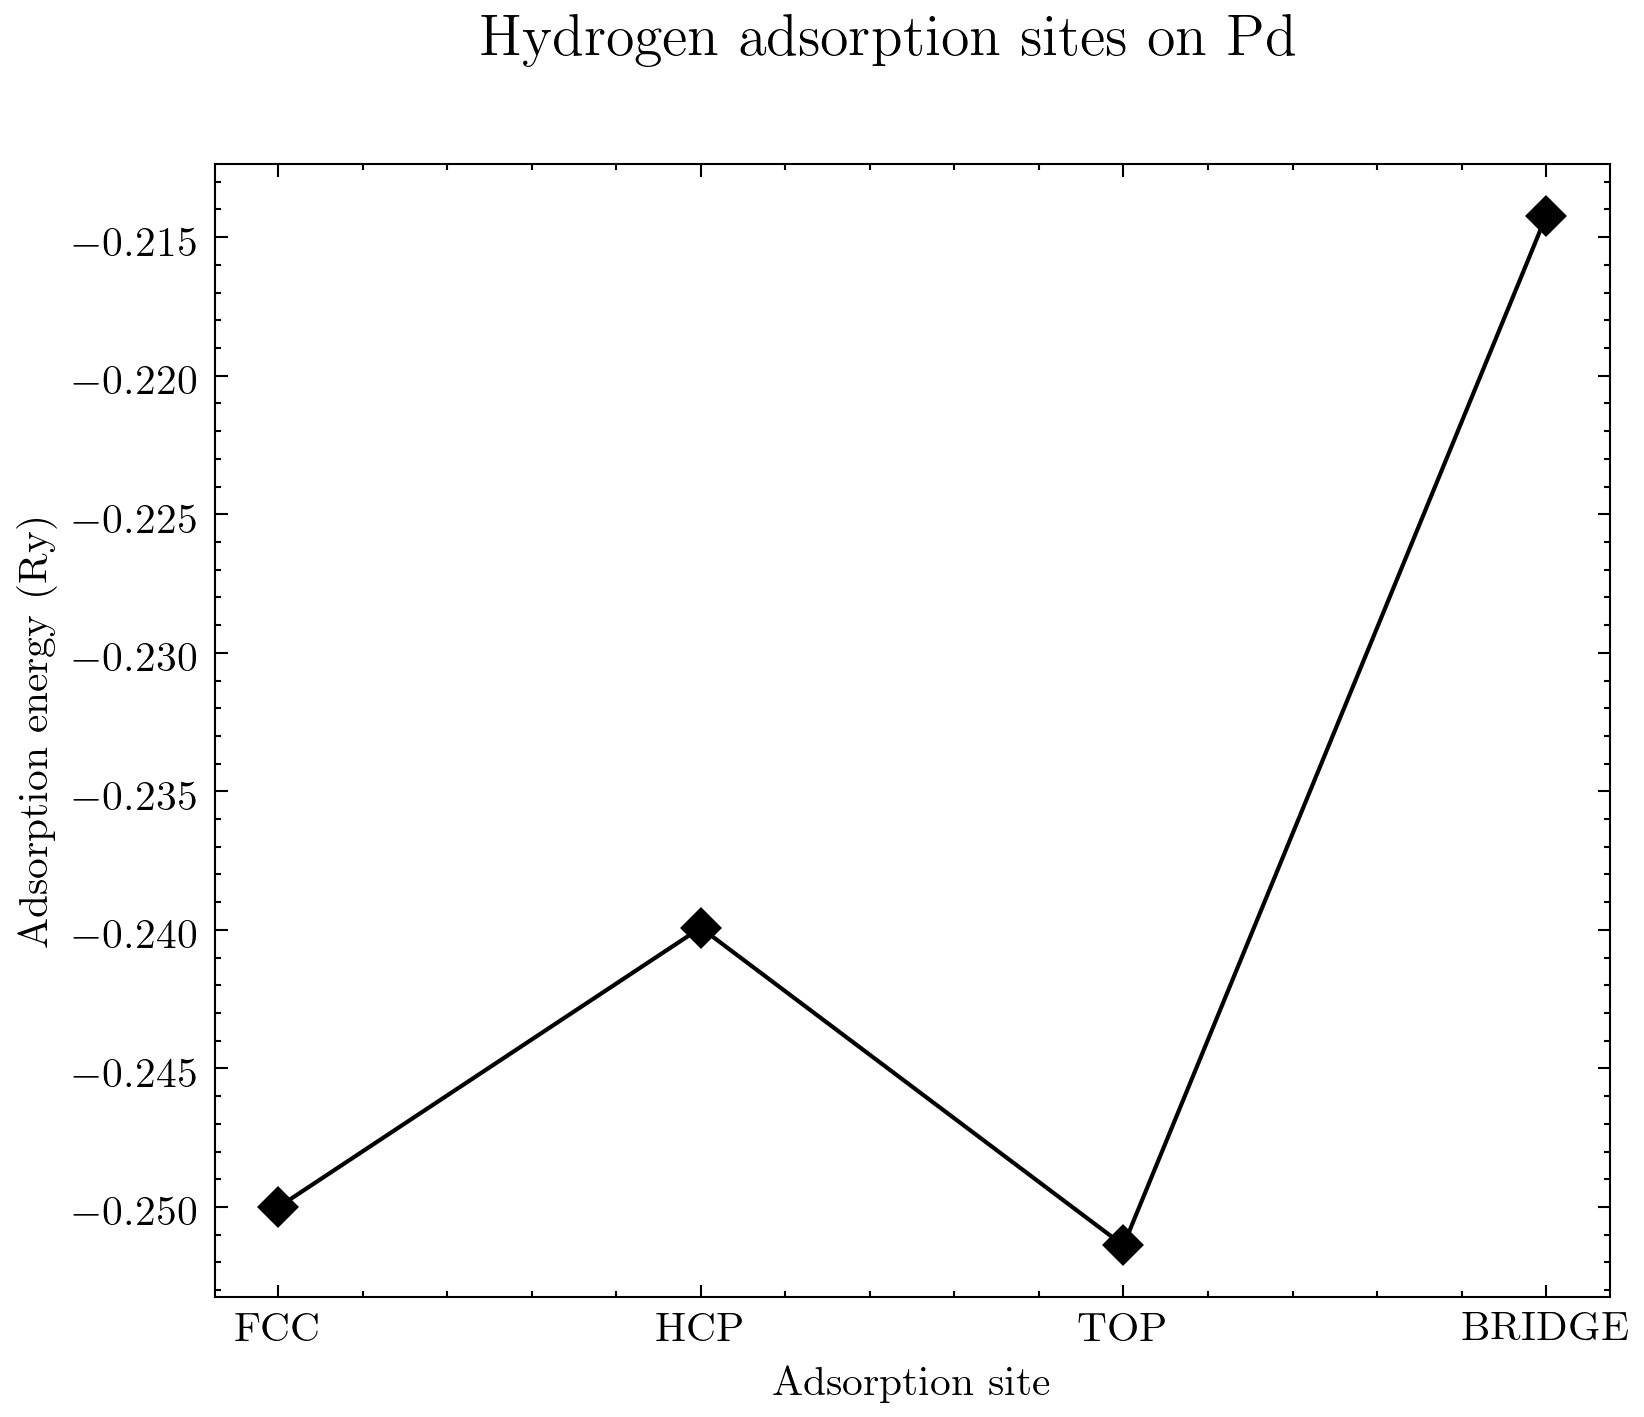
\includegraphics{/Users/marc/Thesis/Chapter3/data/PDSITES.jpg}
  \caption{Adsorption energy of H for each site on a 2x2x5 Pd slab}
  \label{Pdsite}
\end{figure}

All alloys show a decreased preference towards hydrogen binding compared to pure palladium. This is due to hydrogen adsorption energies being closely related to the catalytic activity for hydrogen dissociation of the individual metal elements. The effect appears to be less prevalent for binary alloys with elements with a larger atomic size such as silver which is likely due to the larger atomic size creating a larger area for hydrogen to adsorb within fcc site of the crystalline lattice, which is one of the preferential sites for H adsorption. Zr and Au do not follow this trend however which indicates that the catalytic activity is affected more by electronic interactions than surface geometry. In all cases reduction in palladium from the surface results in lower catalytic activity for hydrogen adsorption which is also likely to be due to the average reduction in number of top sites avaliable for adsorption, which other than FCC is one of the preferential adsorption sites. 

The ternary alloys with the highest catalytic activity were PdAuAg and PdCuAg which previous experimental results showing that these alloys have higher permeability than other ternary alloys. All Zr containing alloys had lower catalytic activity showing that for hydrogen permeation Zr has the greatest inhibiting effect. The detrimental effects of Zr to the catalytic activity can be lowered by the addition of Au, Ag, or Cu however all are still lower than binary alloys. 

The correlation coefficient for the presence of each metal and it's effect on the resulting adsorption energy was calculated and is shown in table \ref{corrH}. It shows that the resulting inhibiting effect of each element follows the order Ag$<$Cu$<$Au$<$Zr. 

This binding energy of hydrogen is an important benchmark for the following tests and will be compared to the resulting binding energies for other impurities. If these impurities show a lower binding energy value when compared to hydrogen then they will be preferntially adsorbed and less suitable for use for that type of impurity. It also reveals that the composition of the membrane can largely effect the catalytic activity for dissociation of hydrogen in itself. As membranes become thinner this will result in a shift of the limiting step to catalytic activity and therefore this value must also be optimised to ensure the highest flux can be achieved, however such work is outside the scope of this study. 

\begin{table}[]
  \centering
  \caption{Correlation coefficient of Ag, Au, Cu, Zr addition to Pd with binding energy of H}
  \label{corrH}
  \begin{tabular}{@{}cc@{}}
  \toprule
  Metal & Correlation coefficient \\ \midrule
  Ag    & -0.024666               \\
  Au    & 0.259205                \\
  Cu    & 0.019221                \\
  Zr    & 0.347930                \\ \bottomrule
  \end{tabular}
  \end{table}

\begin{landscape}
\begin{figure}
    \centering
    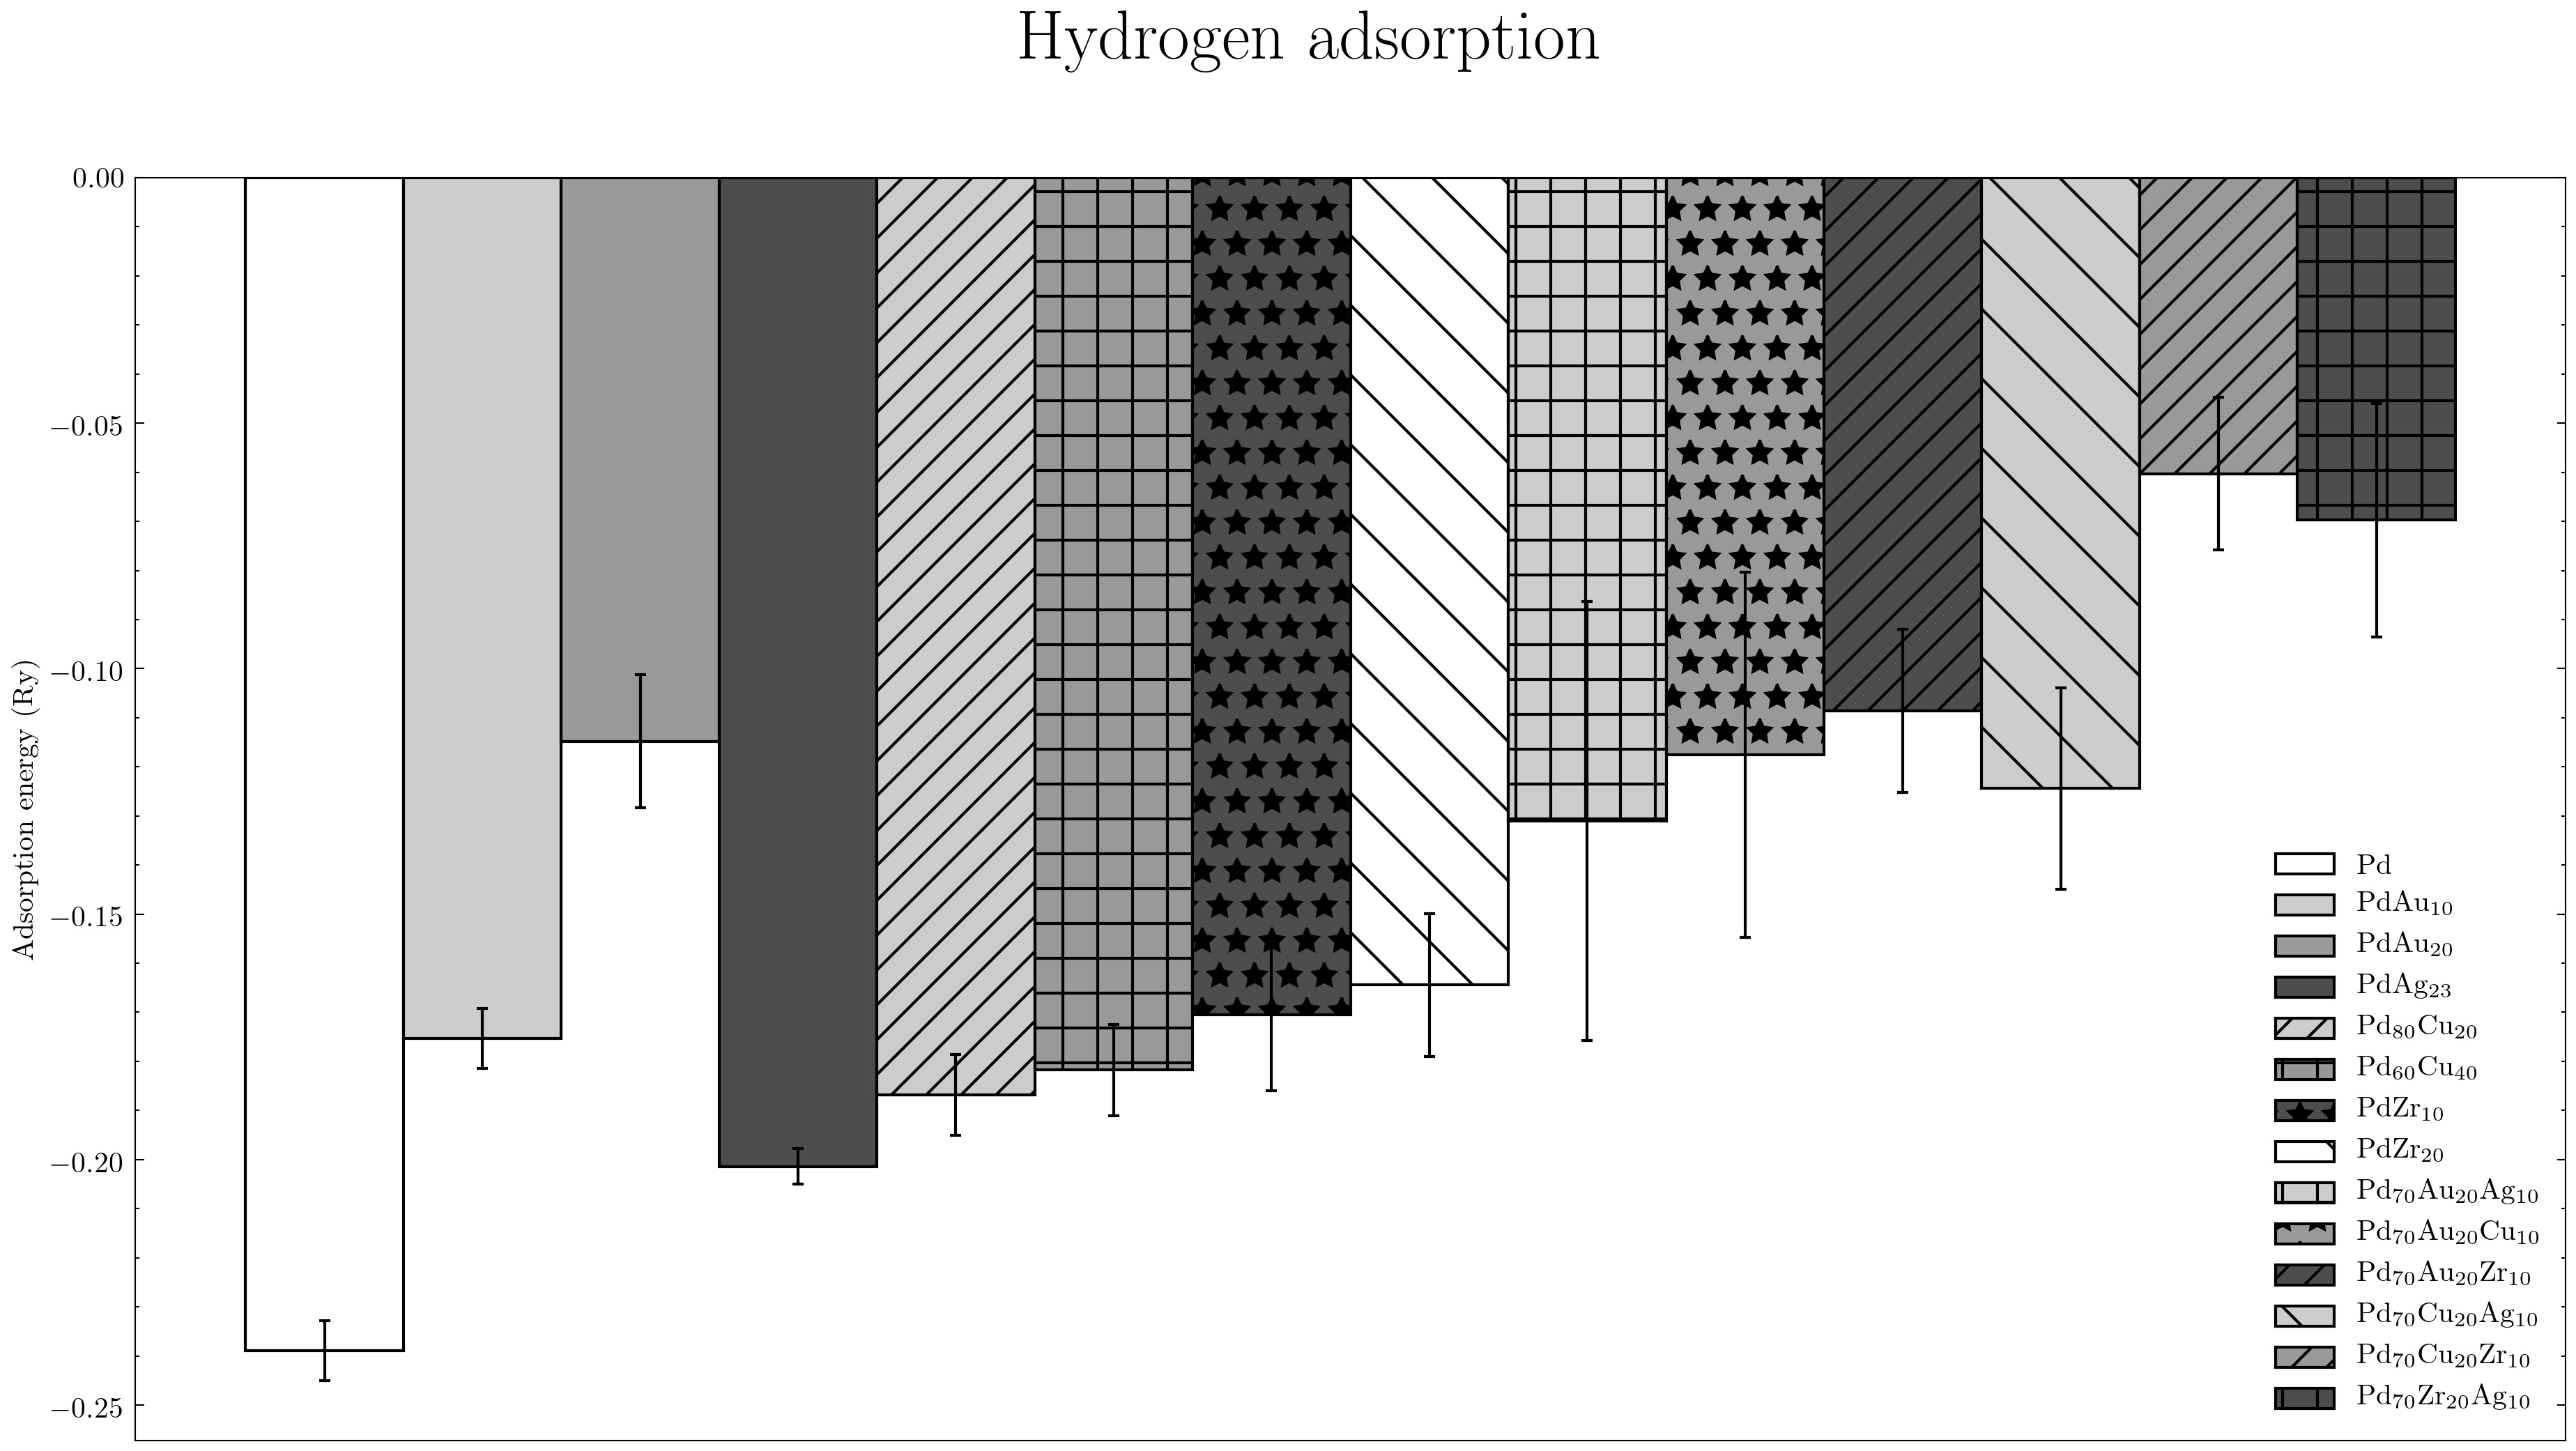
\includegraphics[width=0.9\linewidth,height=\textheight, keepaspectratio]{/Users/marc/Thesis/Chapter3/data/h2ads.jpg}
    \caption{Average binding energy of H\textsubscript{2} on the surface of palladium and palladium alloy slabs}
    \label{h2ads}
  \end{figure}

\end{landscape}
\subsubsection{Helium, Nitrogen, Carbon Dioxide and Argon}
Helium, Nitrogen, Argon, and CO\textsubscript{2} all represent the inert components in fuel cell hydrogen which do not interact with the electrocatalyst and are therefore also likely to be inert to palladium membranes. The binding energies of these molecules on the surface of all the simulated palladium alloy slab systems are shown in figures \ref{heads} (He), \ref{n2ads} (N\textsubscript{2}), \ref{co2ads} (CO\textsubscript{2}) and \ref{Arads} (Ar). All these systems showed a positive binding energy meaning that no competitive adsorption will take place between these gases and hydrogen for the surface adsorption sites.

\begin{figure}
  \centering
  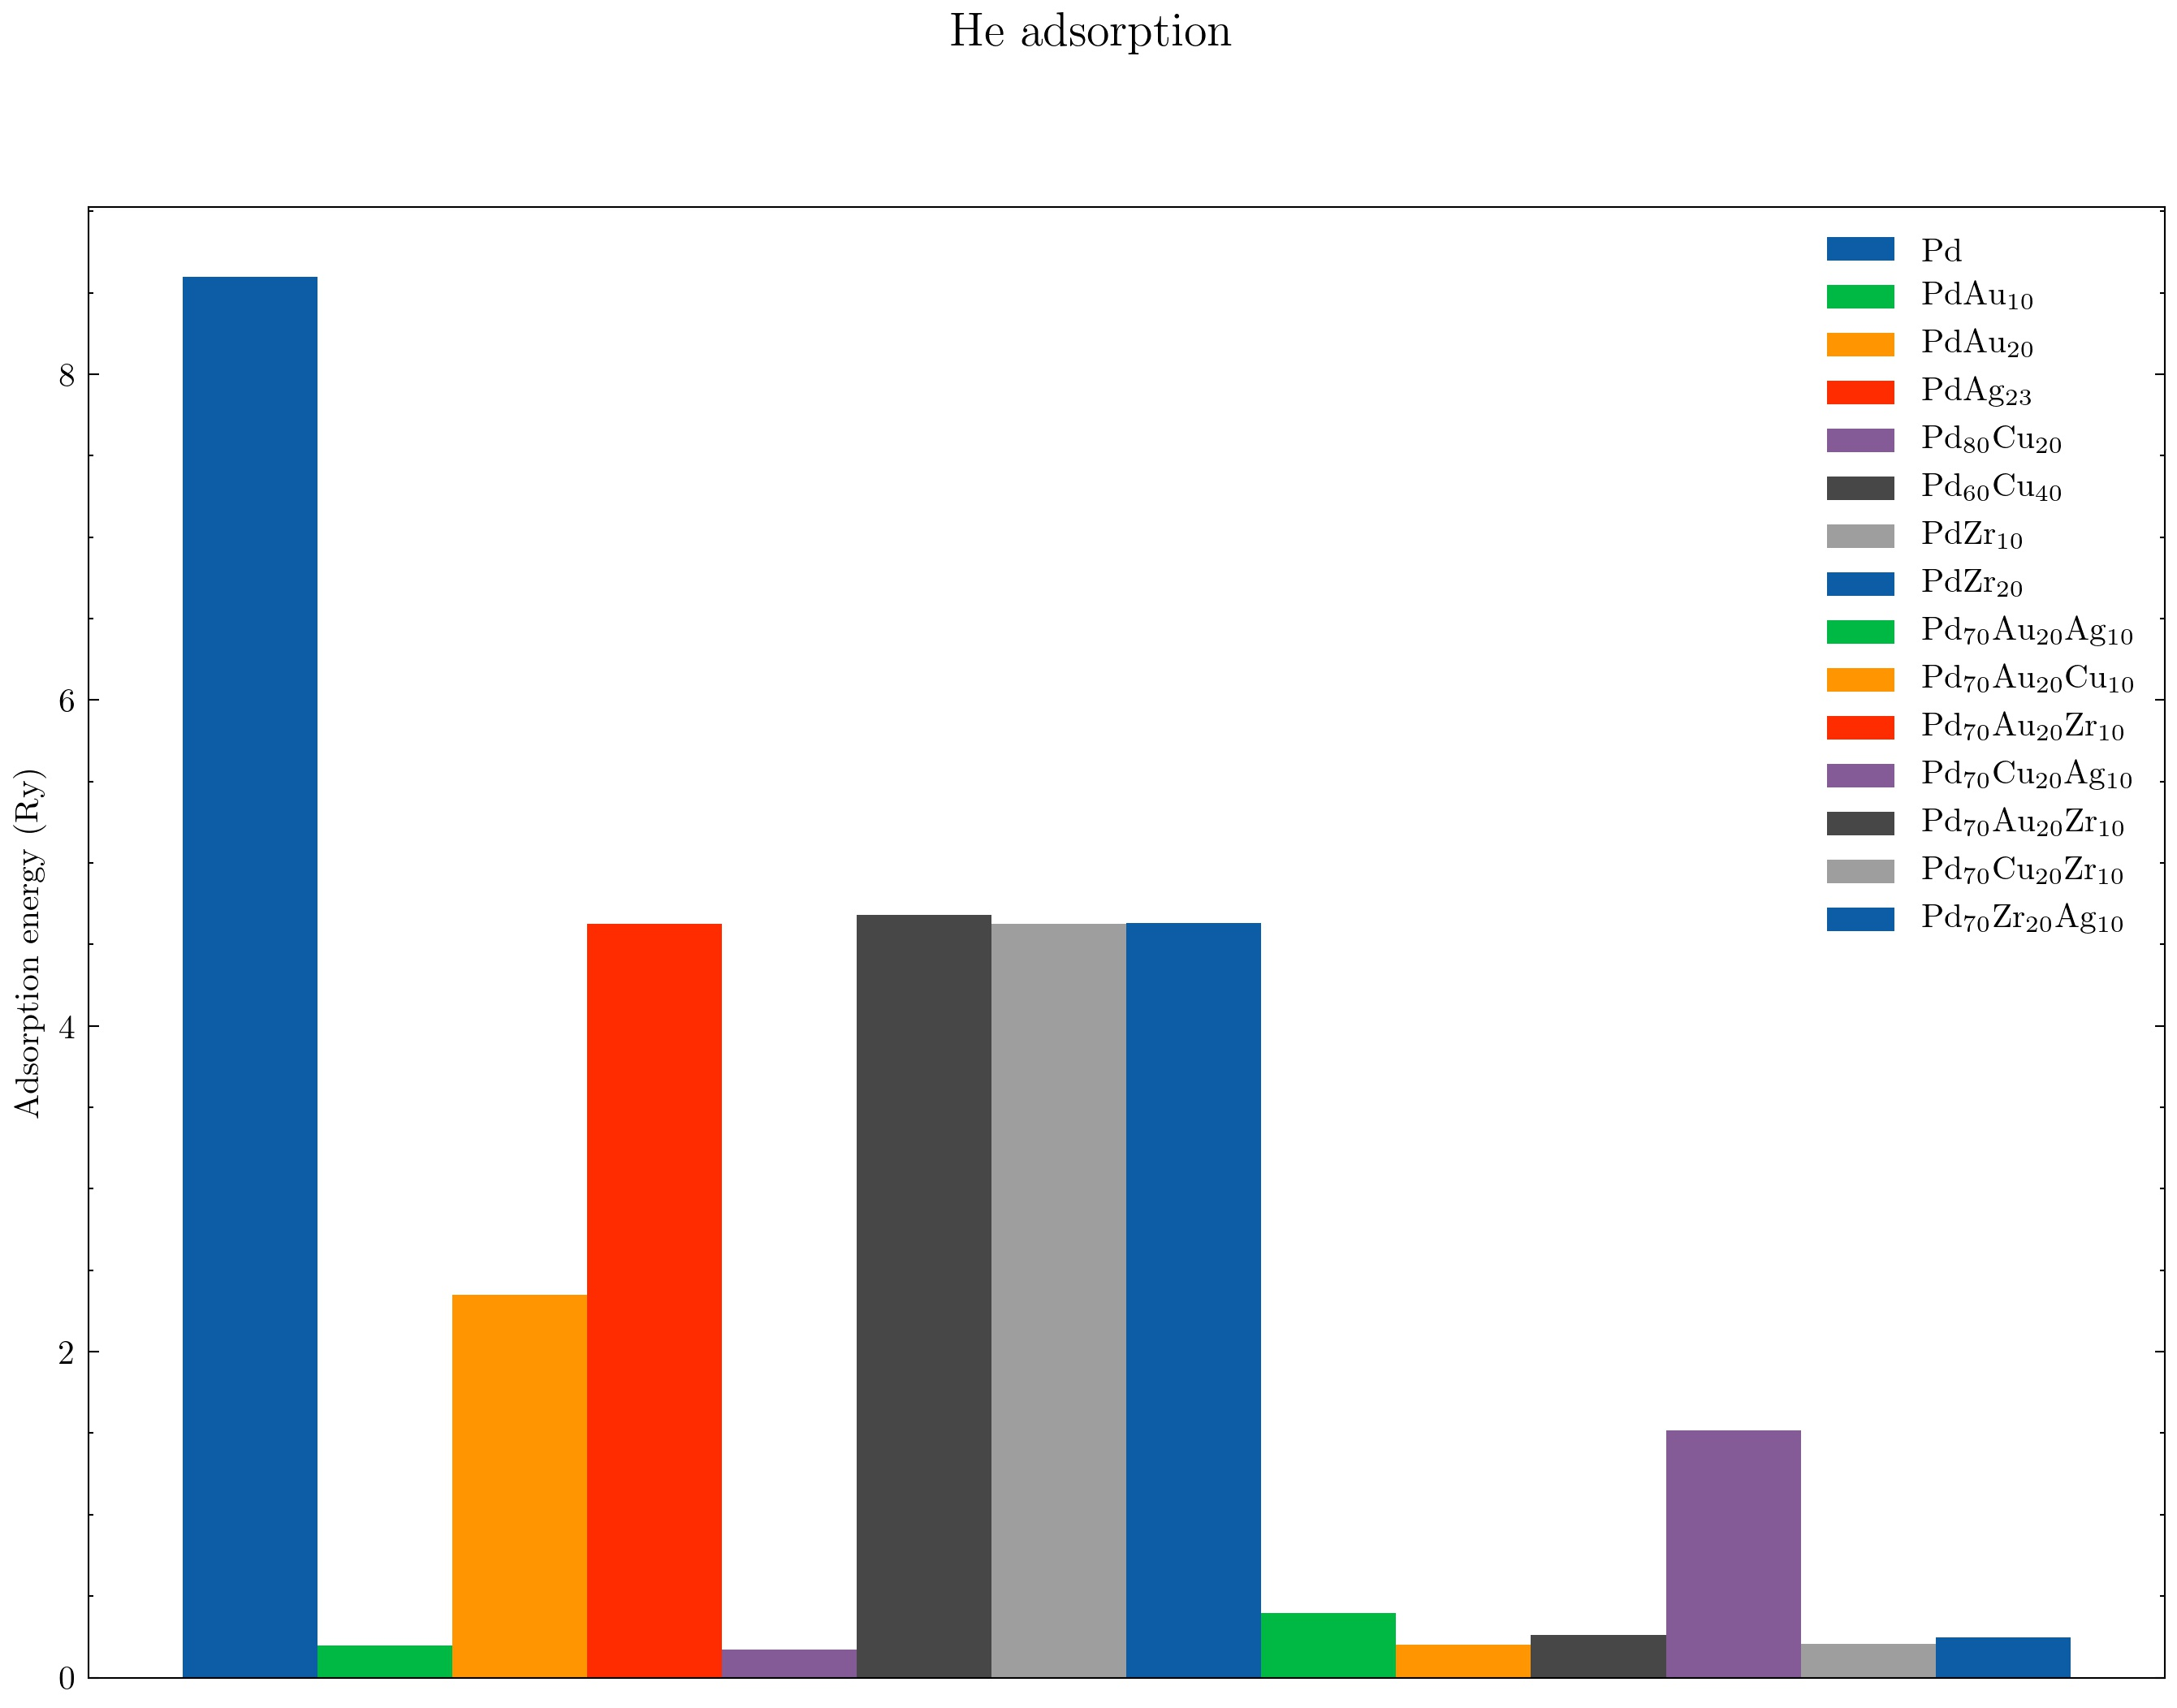
\includegraphics[width=0.9\linewidth, keepaspectratio]{/Users/marc/Thesis/Chapter3/data/HEads.jpg}
  \caption{Average binding energy of He on the surface of palladium and palladium alloy slabs}
  \label{heads}

\end{figure}

    \begin{figure}
        \centering
        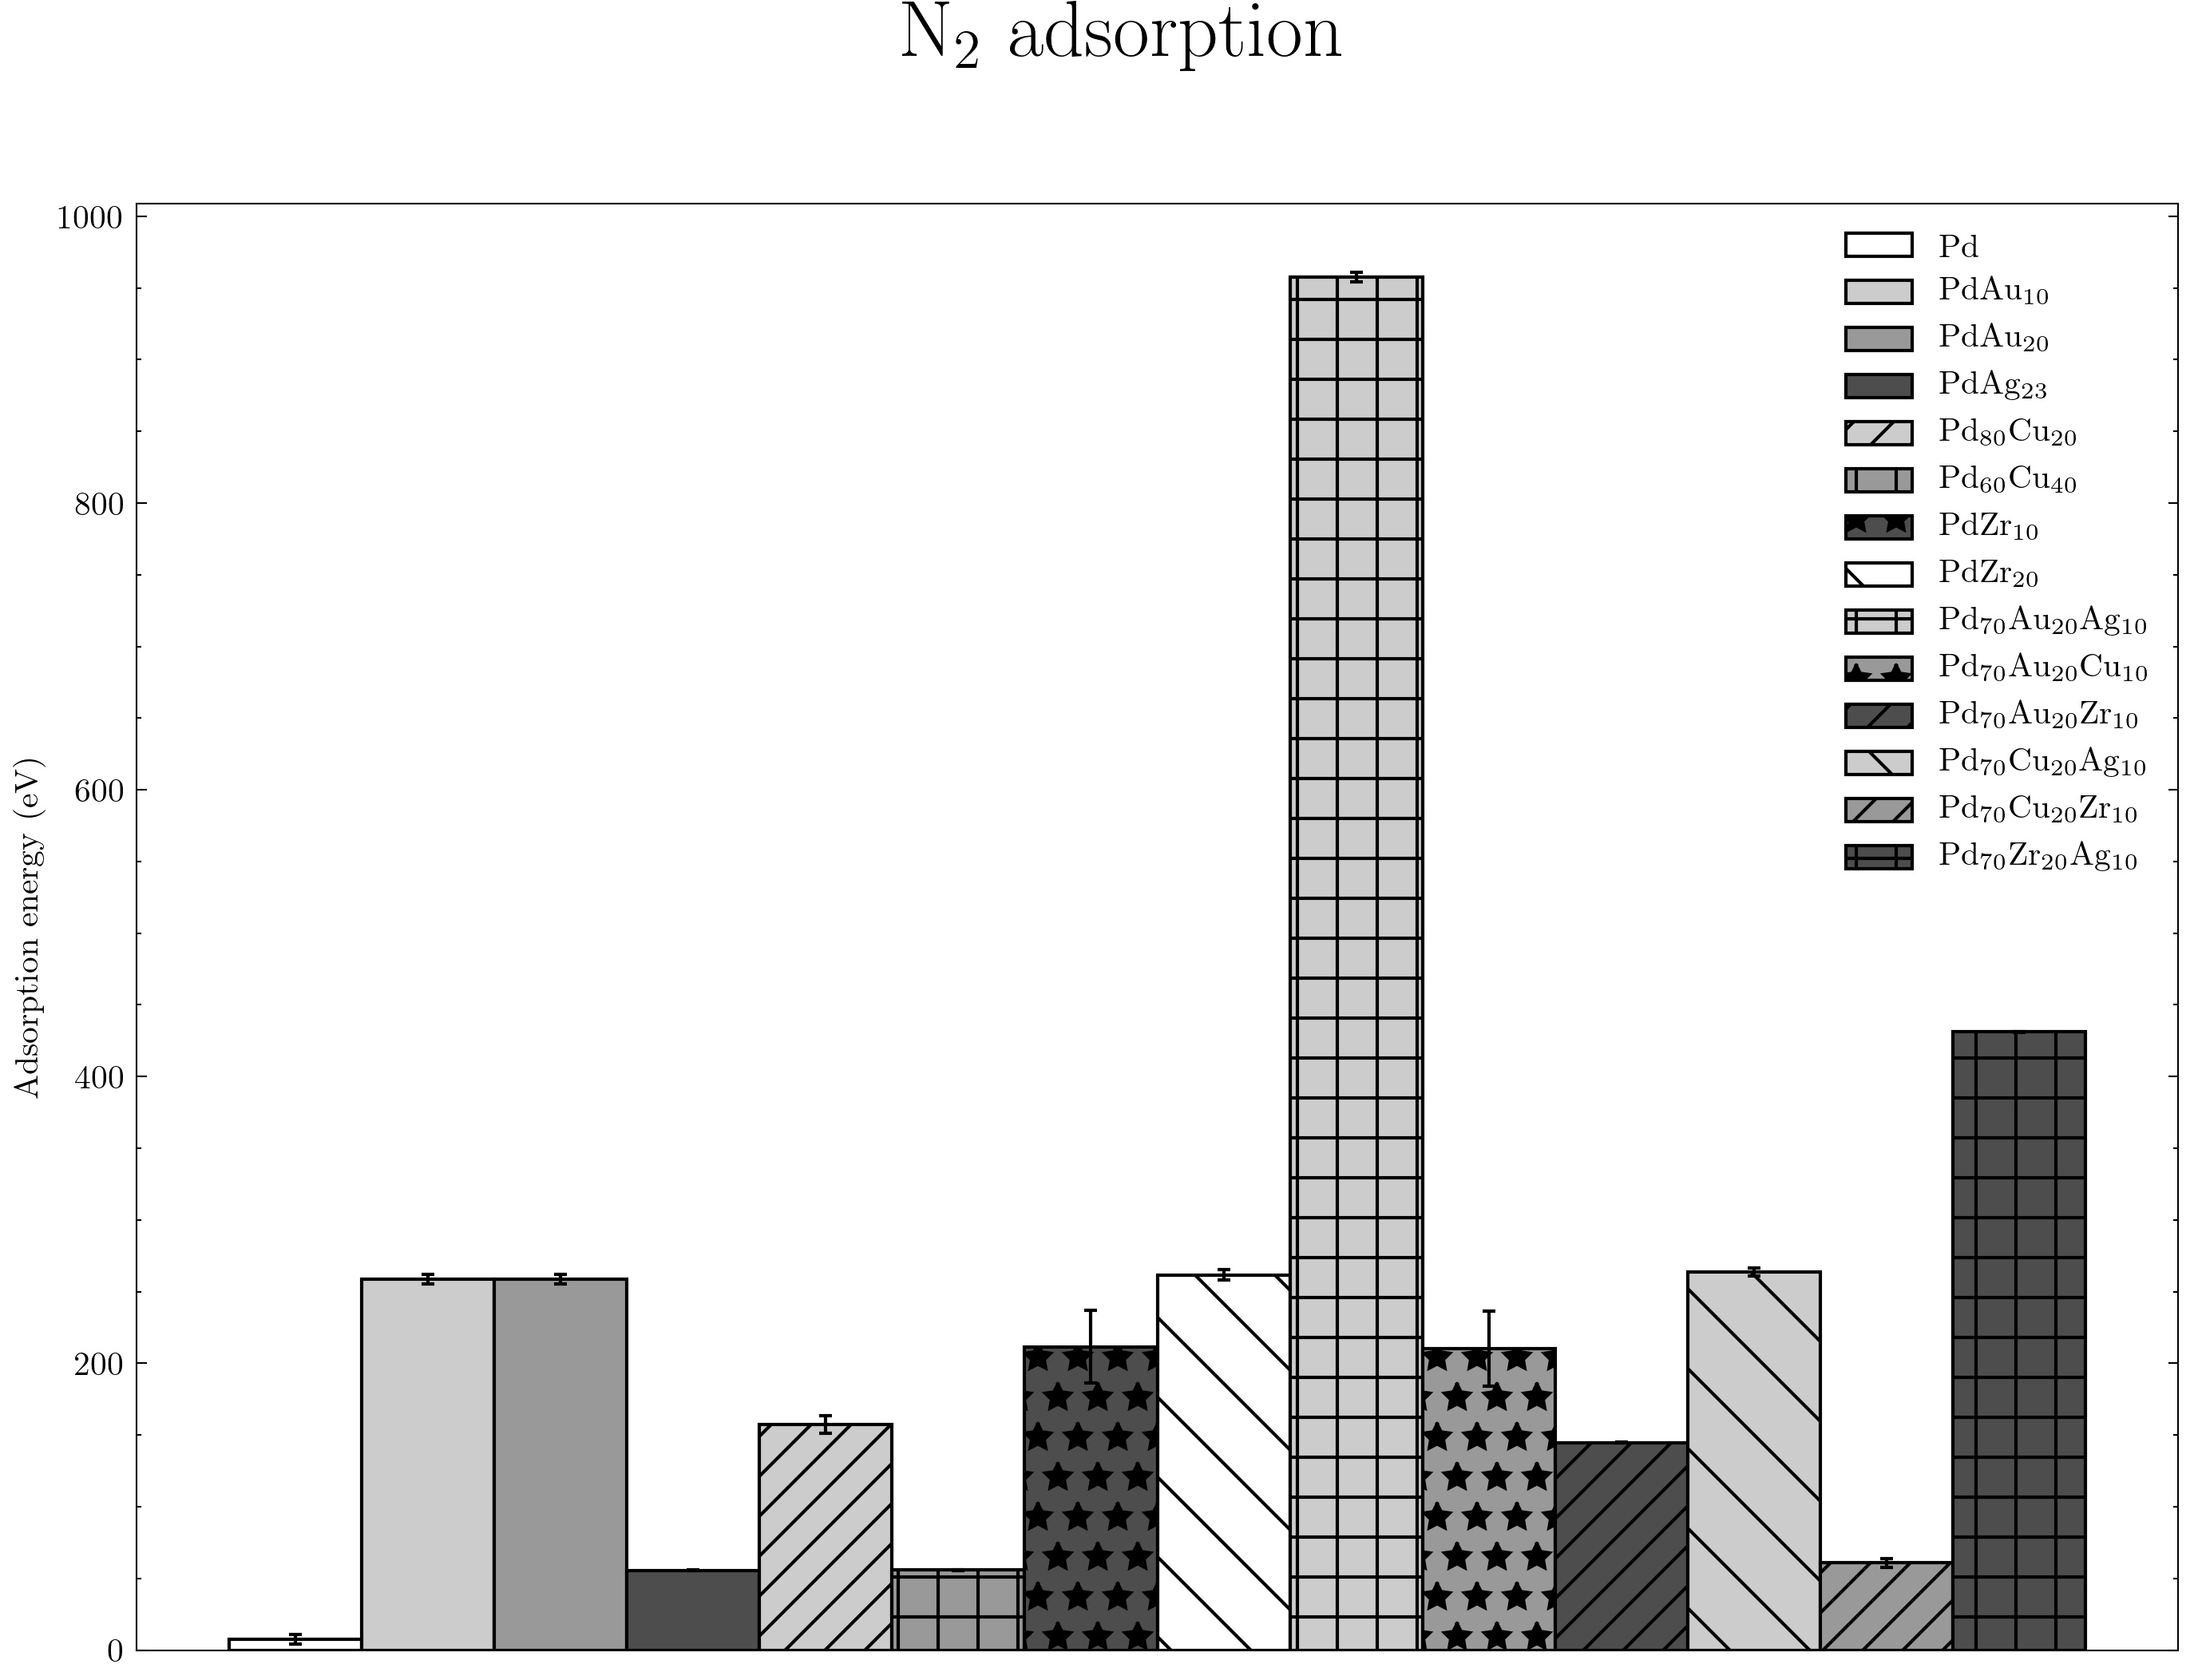
\includegraphics[width=0.9\linewidth, keepaspectratio]{/Users/marc/Thesis/Chapter3/data/N2ads.jpg}
        \caption{Average binding energy of N\textsubscript{2} on the surface of palladium and palladium alloy slabs}
        \label{n2ads}
      \end{figure}

    \begin{figure}
        \centering
        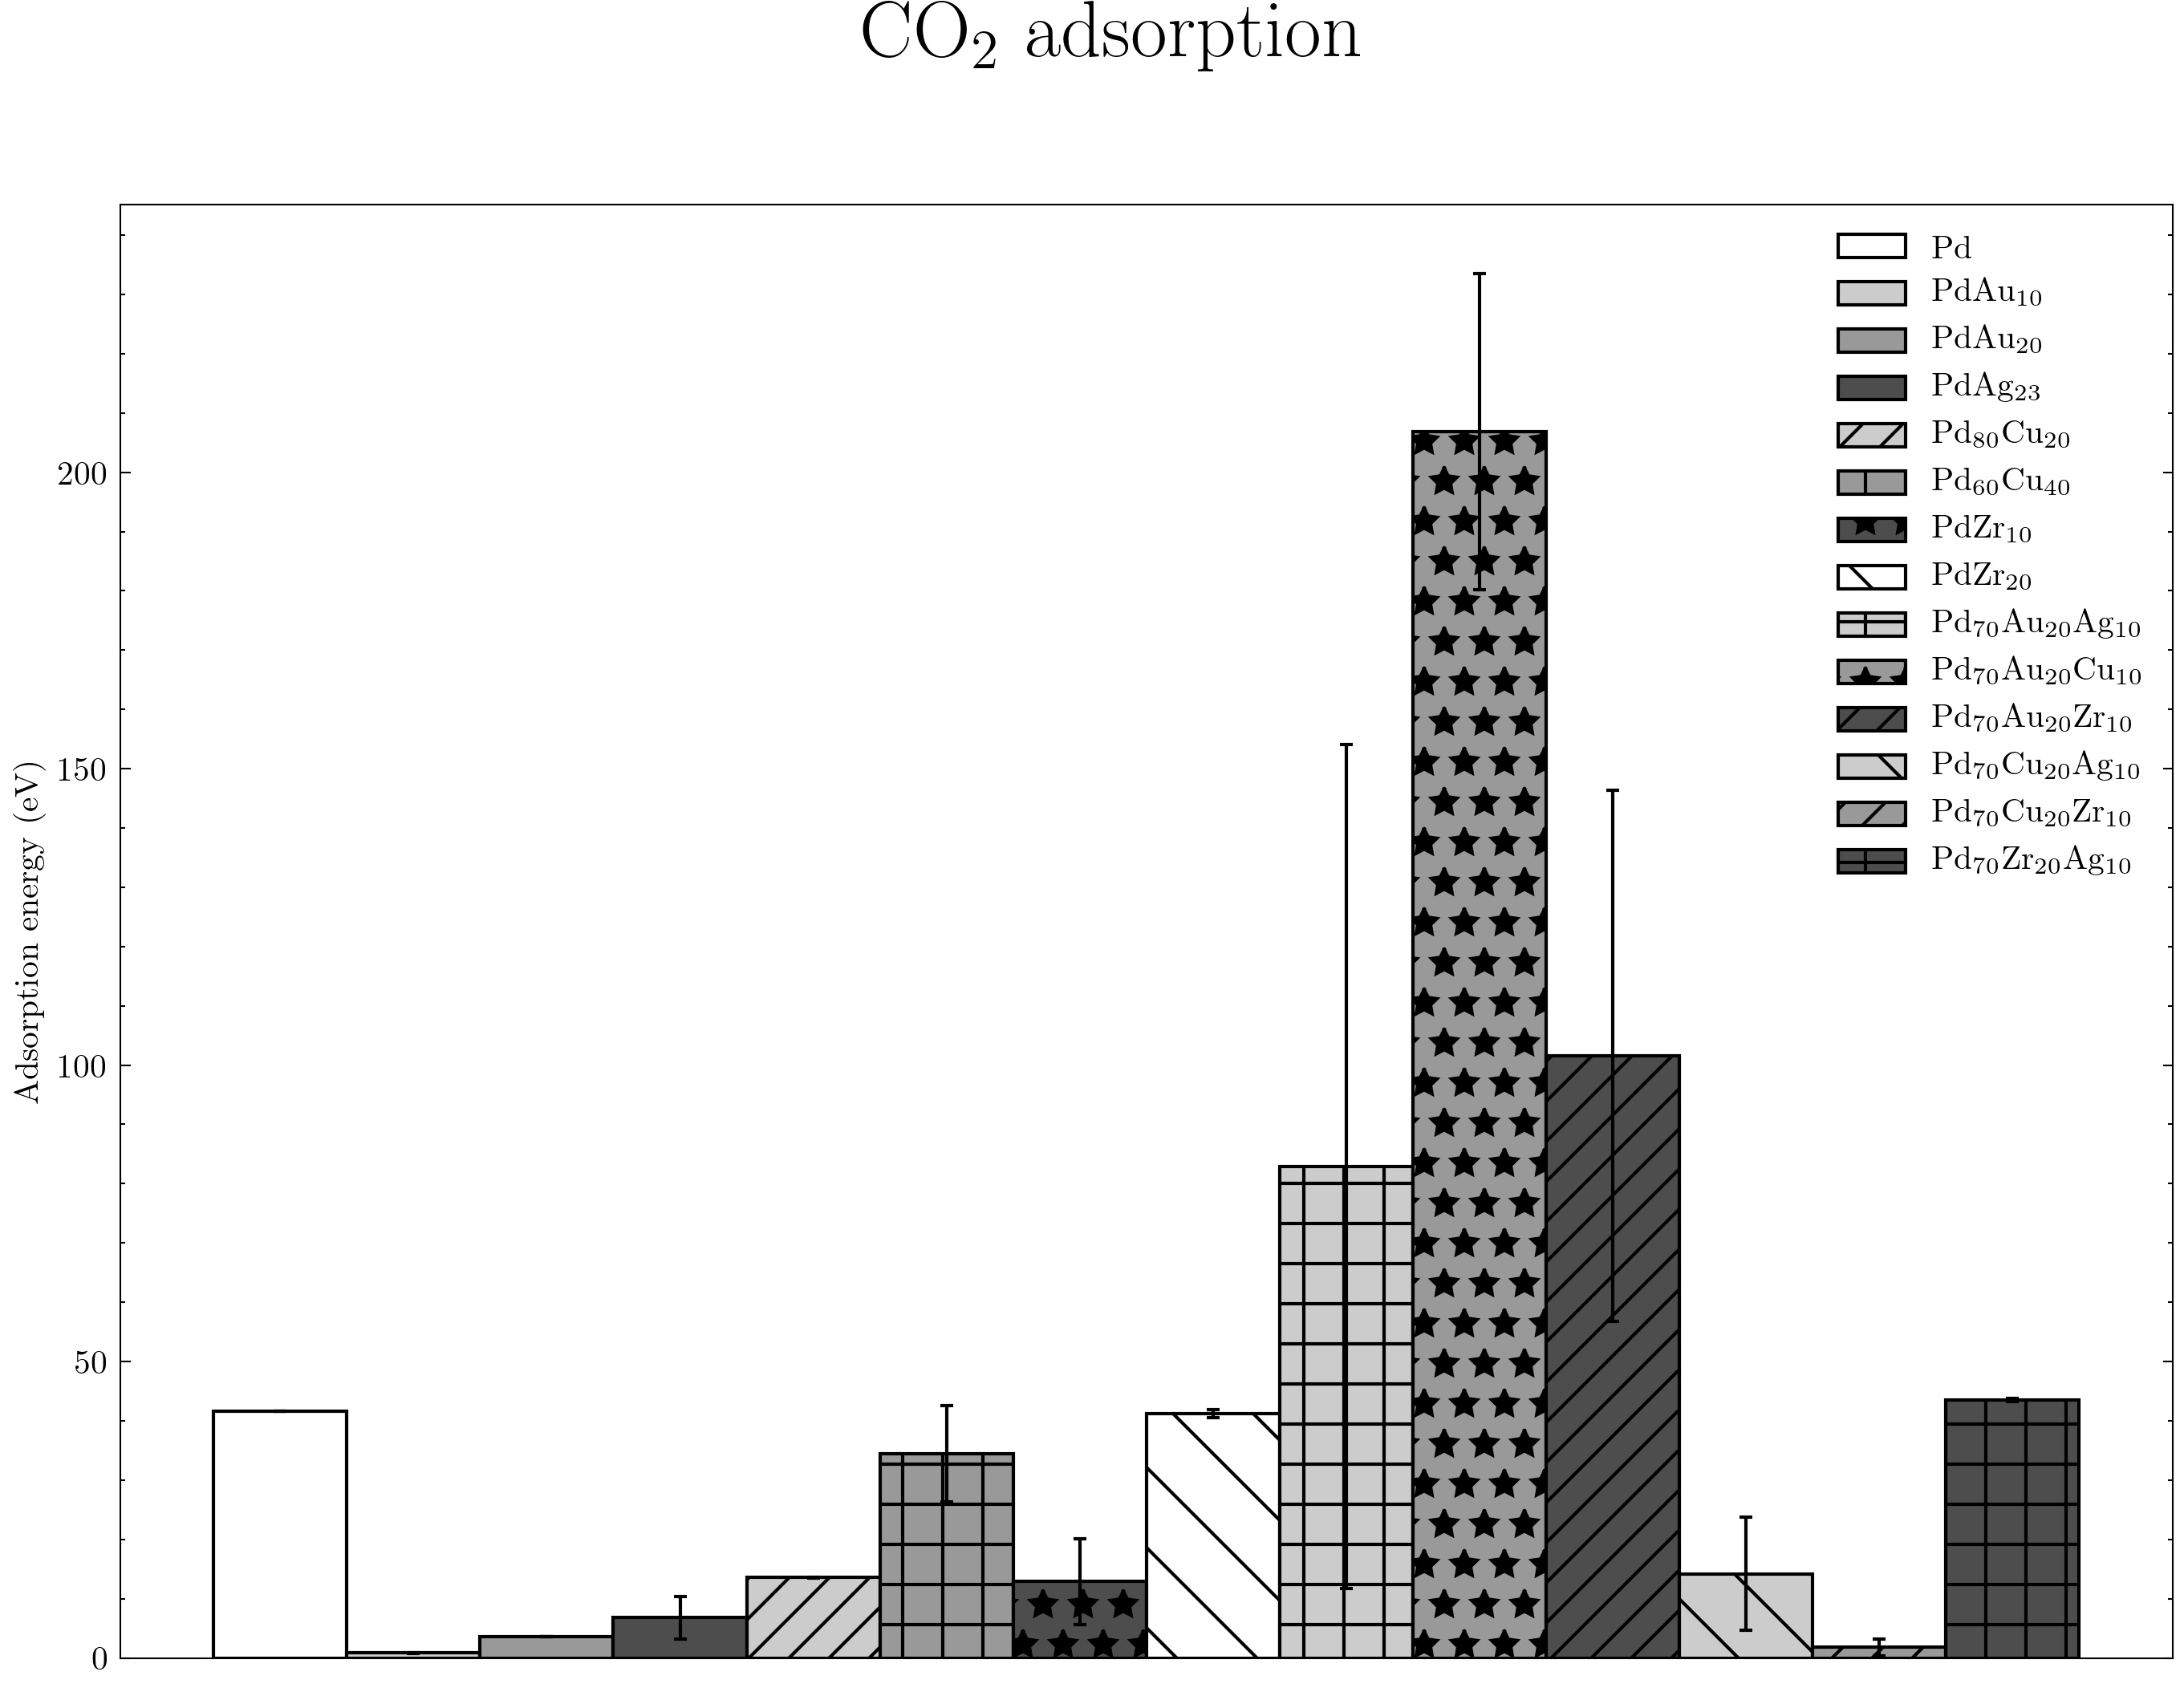
\includegraphics[width=0.9\linewidth, keepaspectratio]{/Users/marc/Thesis/Chapter3/data/CO2ads.jpg}
        \caption{Average binding energy of CO\textsubscript{2} on the surface of palladium and palladium alloy slabs}
        \label{co2ads}
      \end{figure}
    
        \begin{figure}
            \centering
            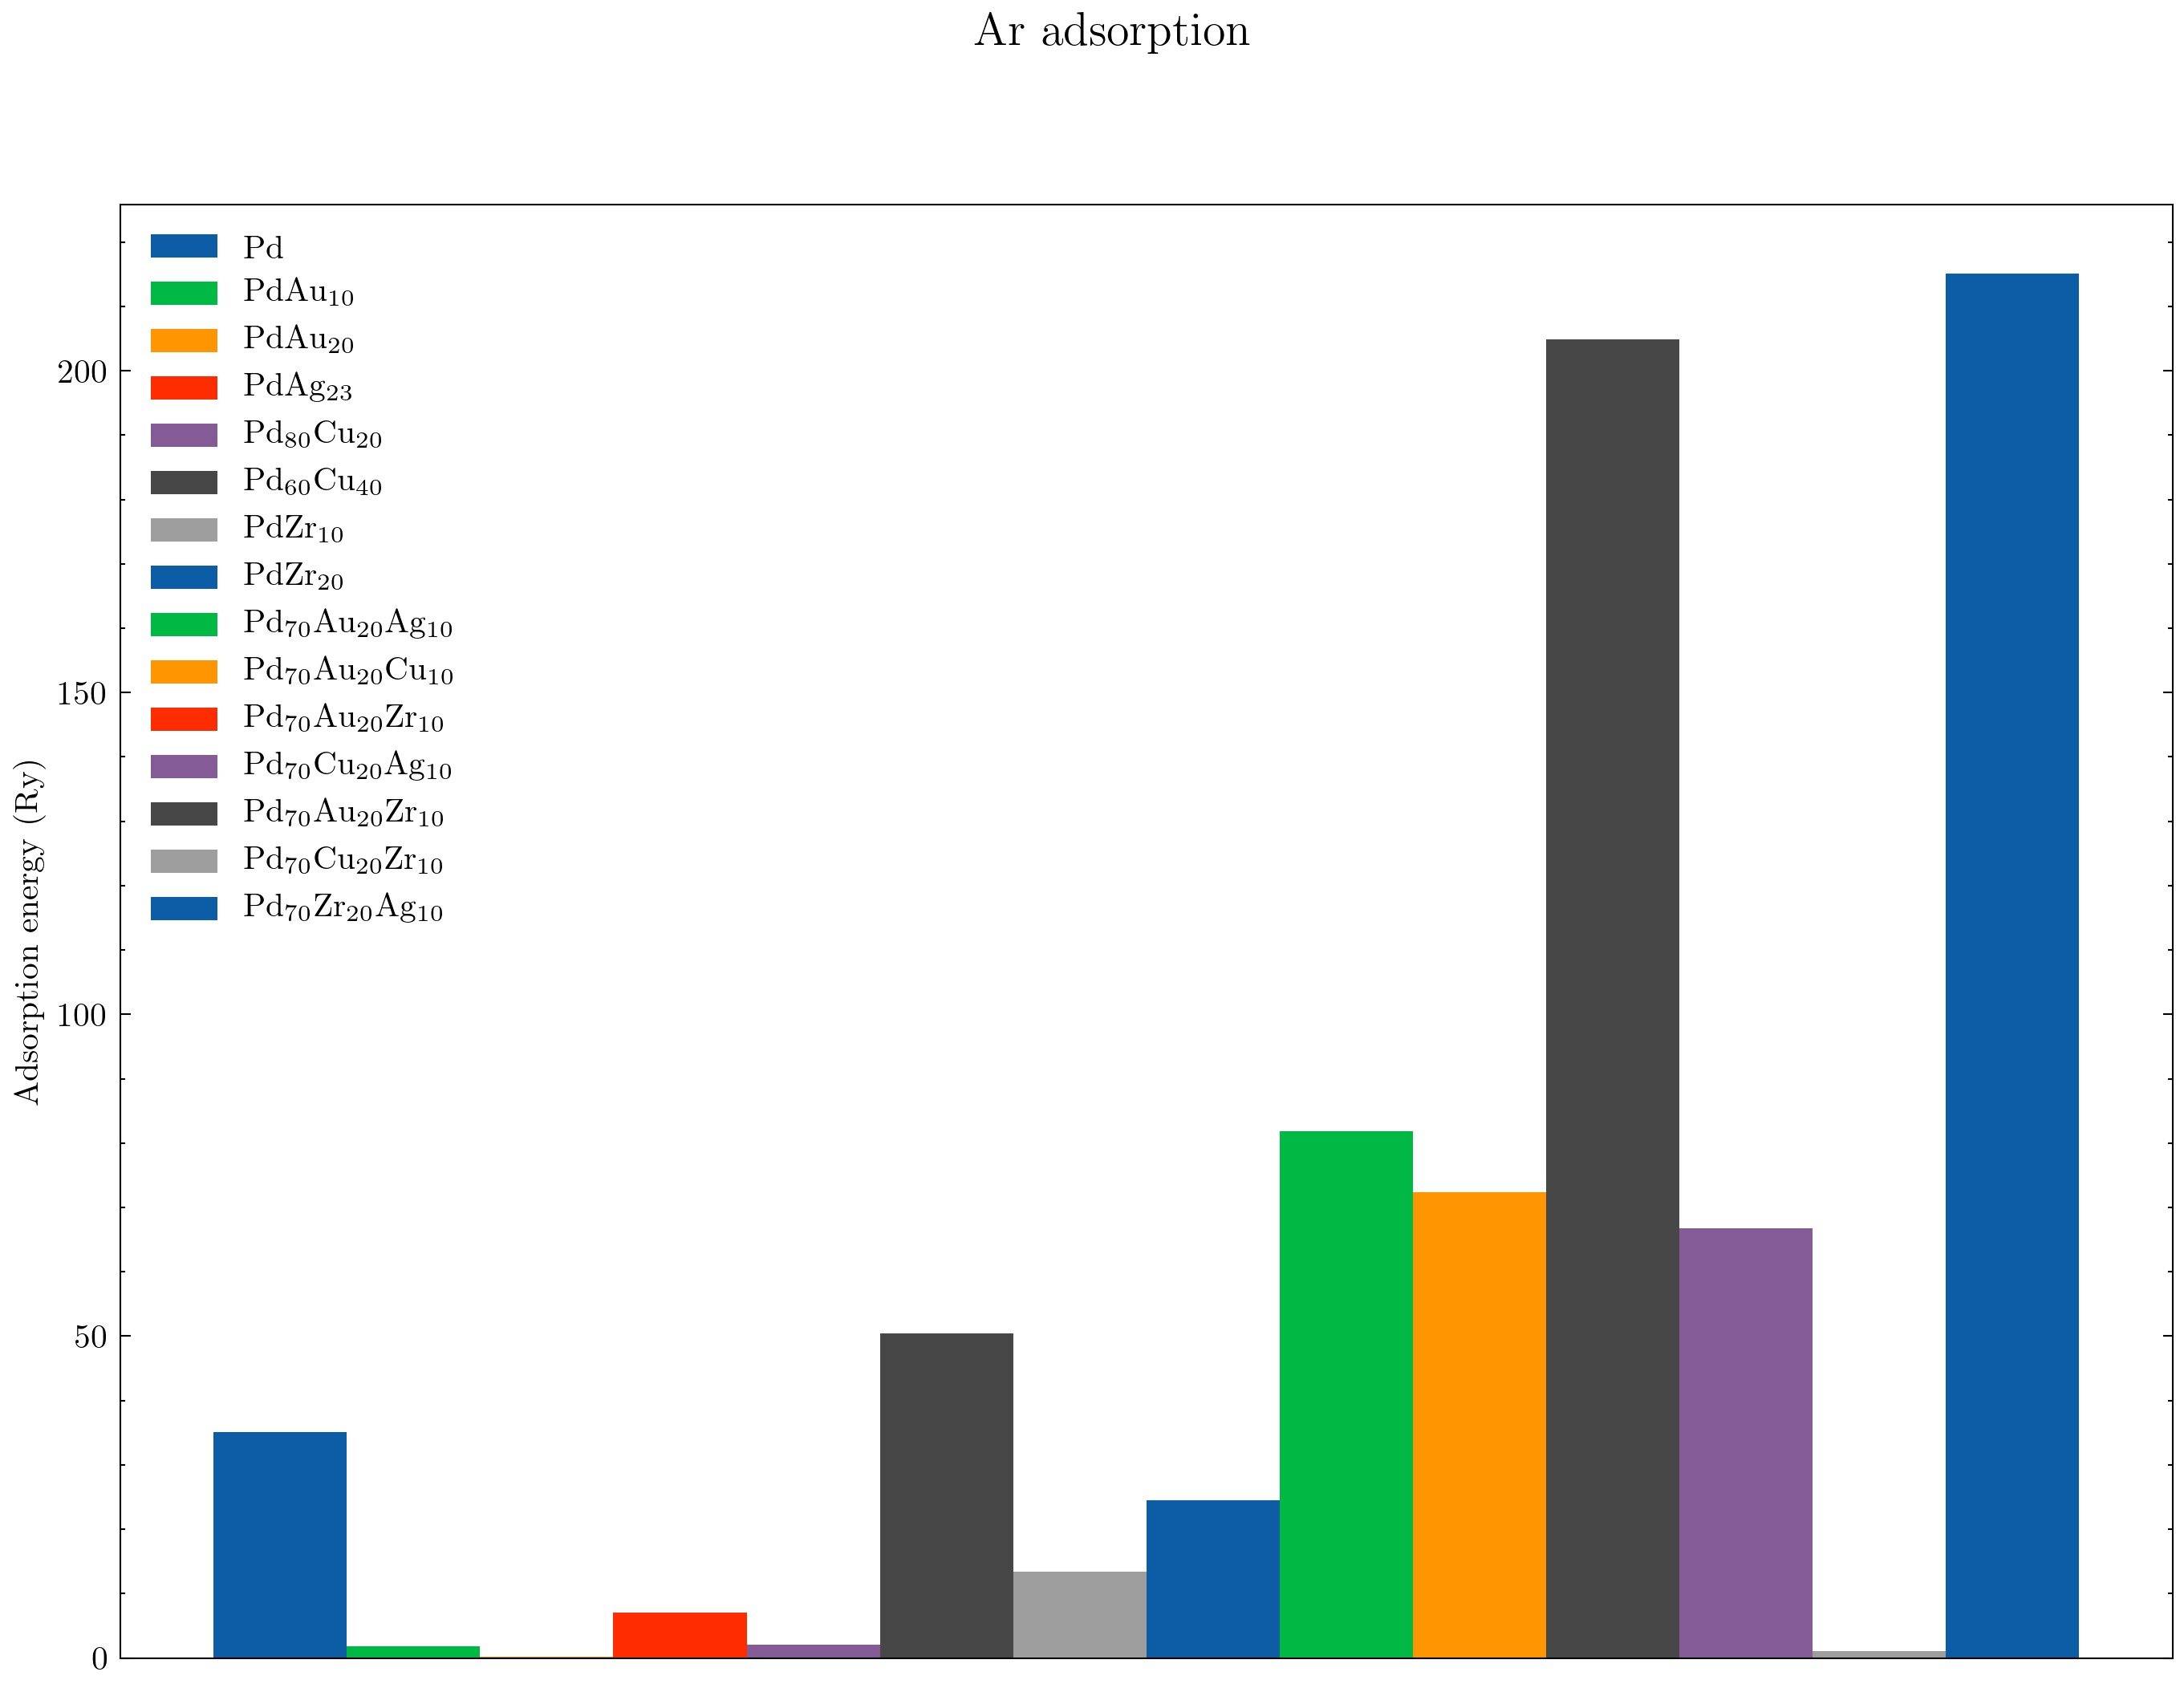
\includegraphics[width=0.9\linewidth, keepaspectratio]{/Users/marc/Thesis/Chapter3/data/ARads.jpg}
            \caption{Average binding energy of Ar on the surface of palladium and palladium alloy slabs}
            \label{Arads}
          \end{figure}
        
\subsubsection{Carbon Monoxide}
CO adsorption was performed by adsorbing the gaseous molecule by the C atom as is normal for CO binding on metallic surfaces \cite{doi:10.1021/acscatal.8b02371}. All systems showed binding preference towards CO. The results of the simulations and their binding energies compared to that of hydrogen on the same alloy are shown in figure \ref{coads}.  No alloys showed an aversion to CO binding therefore all of the simulated alloys, regardless of their preference to H\textsubscript{2}, will likely expereince some competitive adsorption and therefore inhibition when CO is present. 

The pure Pd system showed a clear preference to CO binding over hydrogen, this matches previous experiments performed to investigate this. \cite{Xu2016a} Figure \ref{COsite} shows the binding energy on each site compared to that of H calculated in section \ref{Hsection}. The fcc system shows a clear preference for CO on the FCC, HCP and TOP sites, while still preferring to bind to H on the BRIDGE site. This is most prevalent for the FCC site which has a lower binding energy of around -0.55 eV, with HCP and TOP sites showing a drop in around -0.35 and -0.3 eV respectivley. However since the top site still shows a preference for H binding which represents around 41\% of the binding sites. While this may indicate that these sites are still avaliable for hydrogen permeation, when bulk diffusion is modelled using kinetic monte carlo simulations that hydrogen travels through the bulk by relaxing the lattice around the fcc and hcp sites to facilitate transport. \cite{Qin2012} Therefore the blocking of these sites is likely to have a severe effect on hydrogen permeation.

Of the systems tested PdAu\textsubscript{20}, PdAg\textsubscript{23}, and Pd\textsubscript{70}Au\textsubscript{20}Cu\textsubscript{10} all showed marginal preference for hydrogen binding over CO binding. Binding of CO on Au and Ag surfaces has previously been studied and concluded that these metals do not interact with CO under normal circumstances, and will only adsorb through way of material defect or alloying. \cite{doi:10.1021/la950167j} \cite{shaikhutdinov_meyer_naschitzki_baumer_freund_2003}

By far the worst performing metal for inhibiting the effect of CO were all Zr containing alloys, and Pd\textsubscript{60}Cu\textsubscript{40}. Zr readily forms a bond with C, and even has it's own unique branch of chemistry referring to such compounds.\cite{doi:10.1021/cen-v082n016.p036} Zirconium is also a common complex used in homogeneous refactory catalysts for reforming hydrocarbon compounds.\cite{doi:10.1002/9780470504437.ch1} Therefore the evidence suggests that Zr naturally has a high affinity towards forming carbon bonds and is not a suitable additive for CO resistent membranes. 

Similarly Cu has been previously studied and found to readily adsorb CO on it's surface. \cite{doi:10.1021/la950167j} This does not appear to be an issue for PdCu\textsubscript{20} alloys indicating that this level of Cu is too low to have such an effect. The Pd\textsubscript{60}Cu\textsubscript{40} alloy on the other hand has a much higher binding prefernce for CO than it's sister hydrogen system. Pd\textsubscript{60}Cu\textsubscript{40} is different from other systems in that the crystalline structure transitions to a BCC lattice. \cite{She2014} BCC structures only have two different sites avaliable for hydrogen binding, BRIDGE and HCP. \cite{C3CP44367A} This change in structure combined with the Cu's avalability to bind with C likely accounts for the large discrepancy. 

\begin{figure}
  \centering
  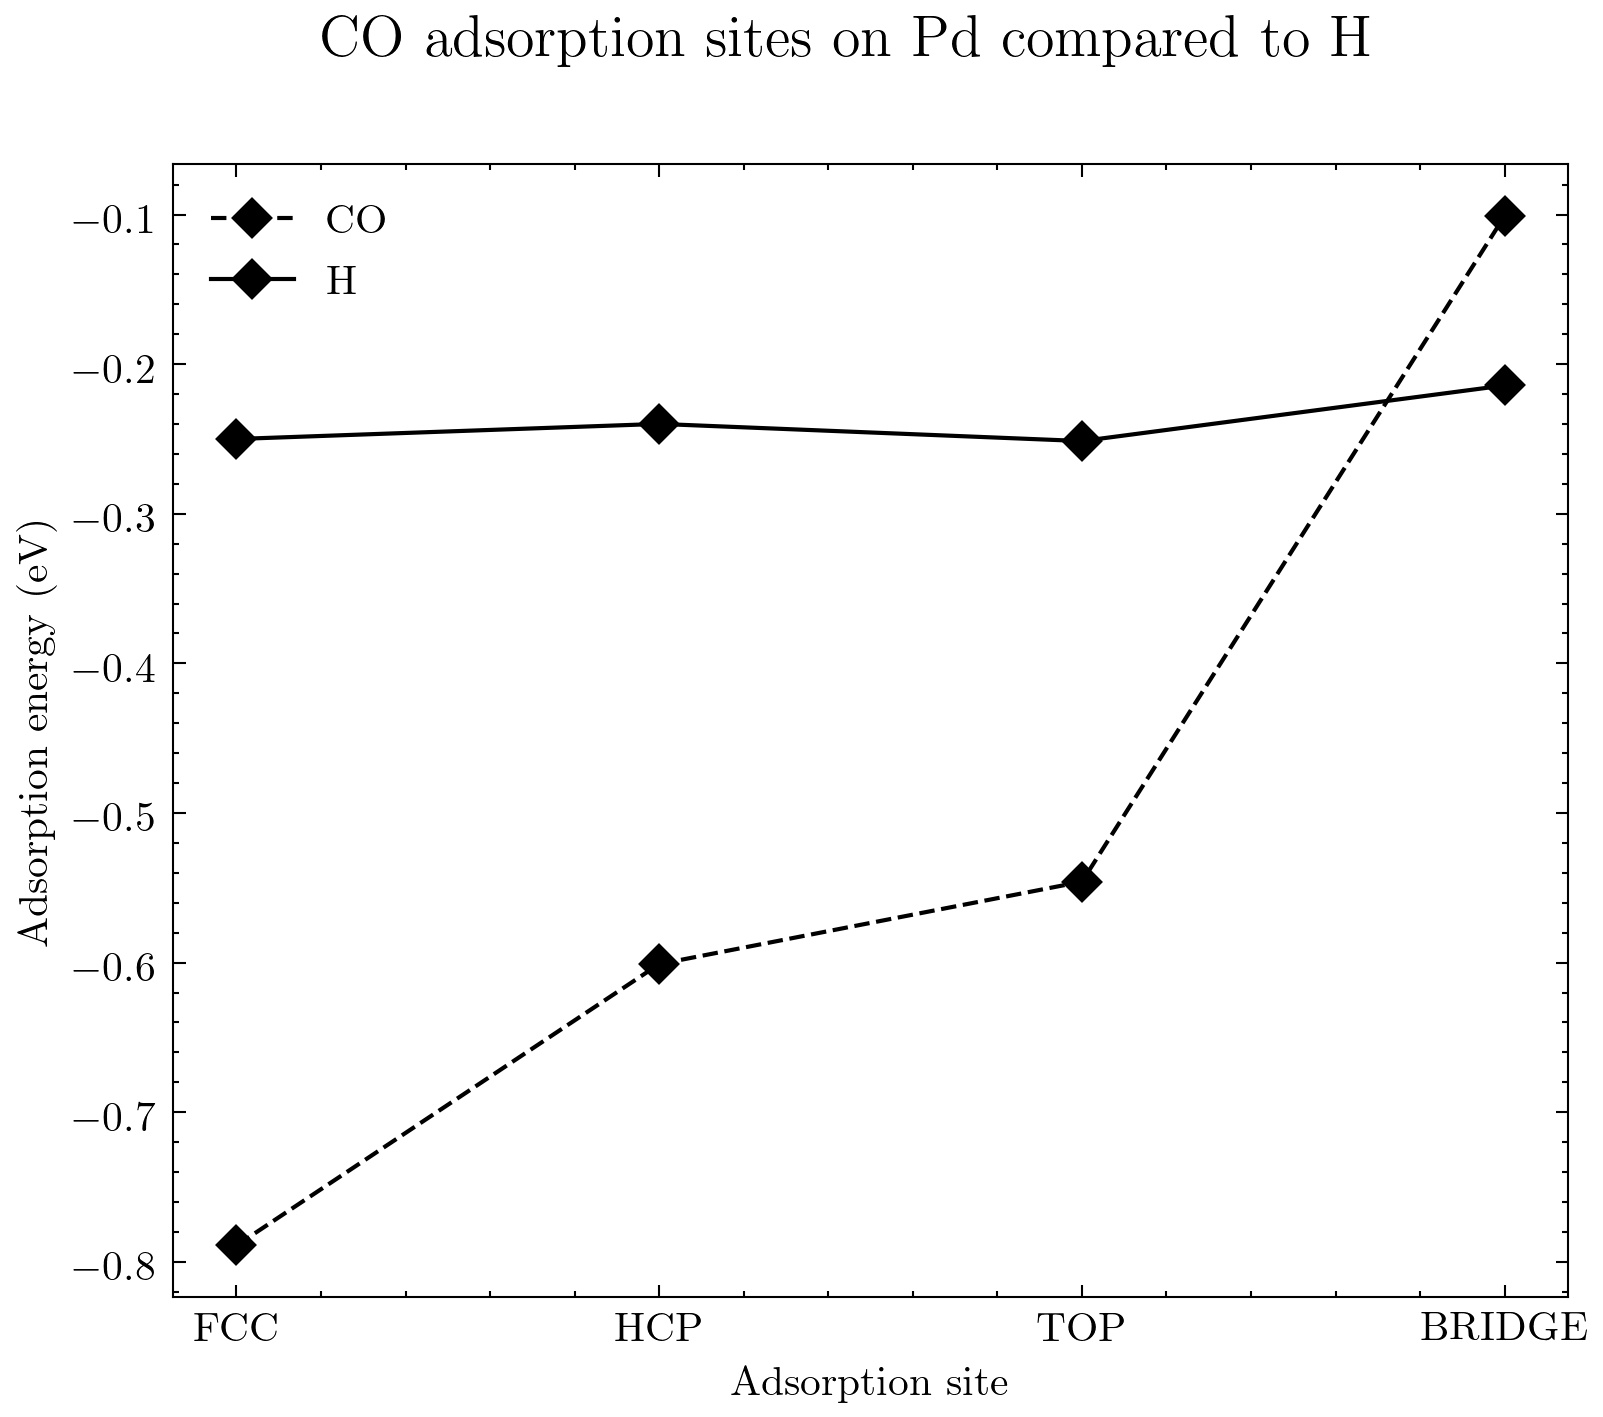
\includegraphics{/Users/marc/Thesis/Chapter3/data/COSites.jpg}
  \caption{binding energy of H and CO for each site on a 2x2x5 Pd slab}
  \label{COsite}
\end{figure}


\begin{landscape}
    \begin{figure}
        \centering
        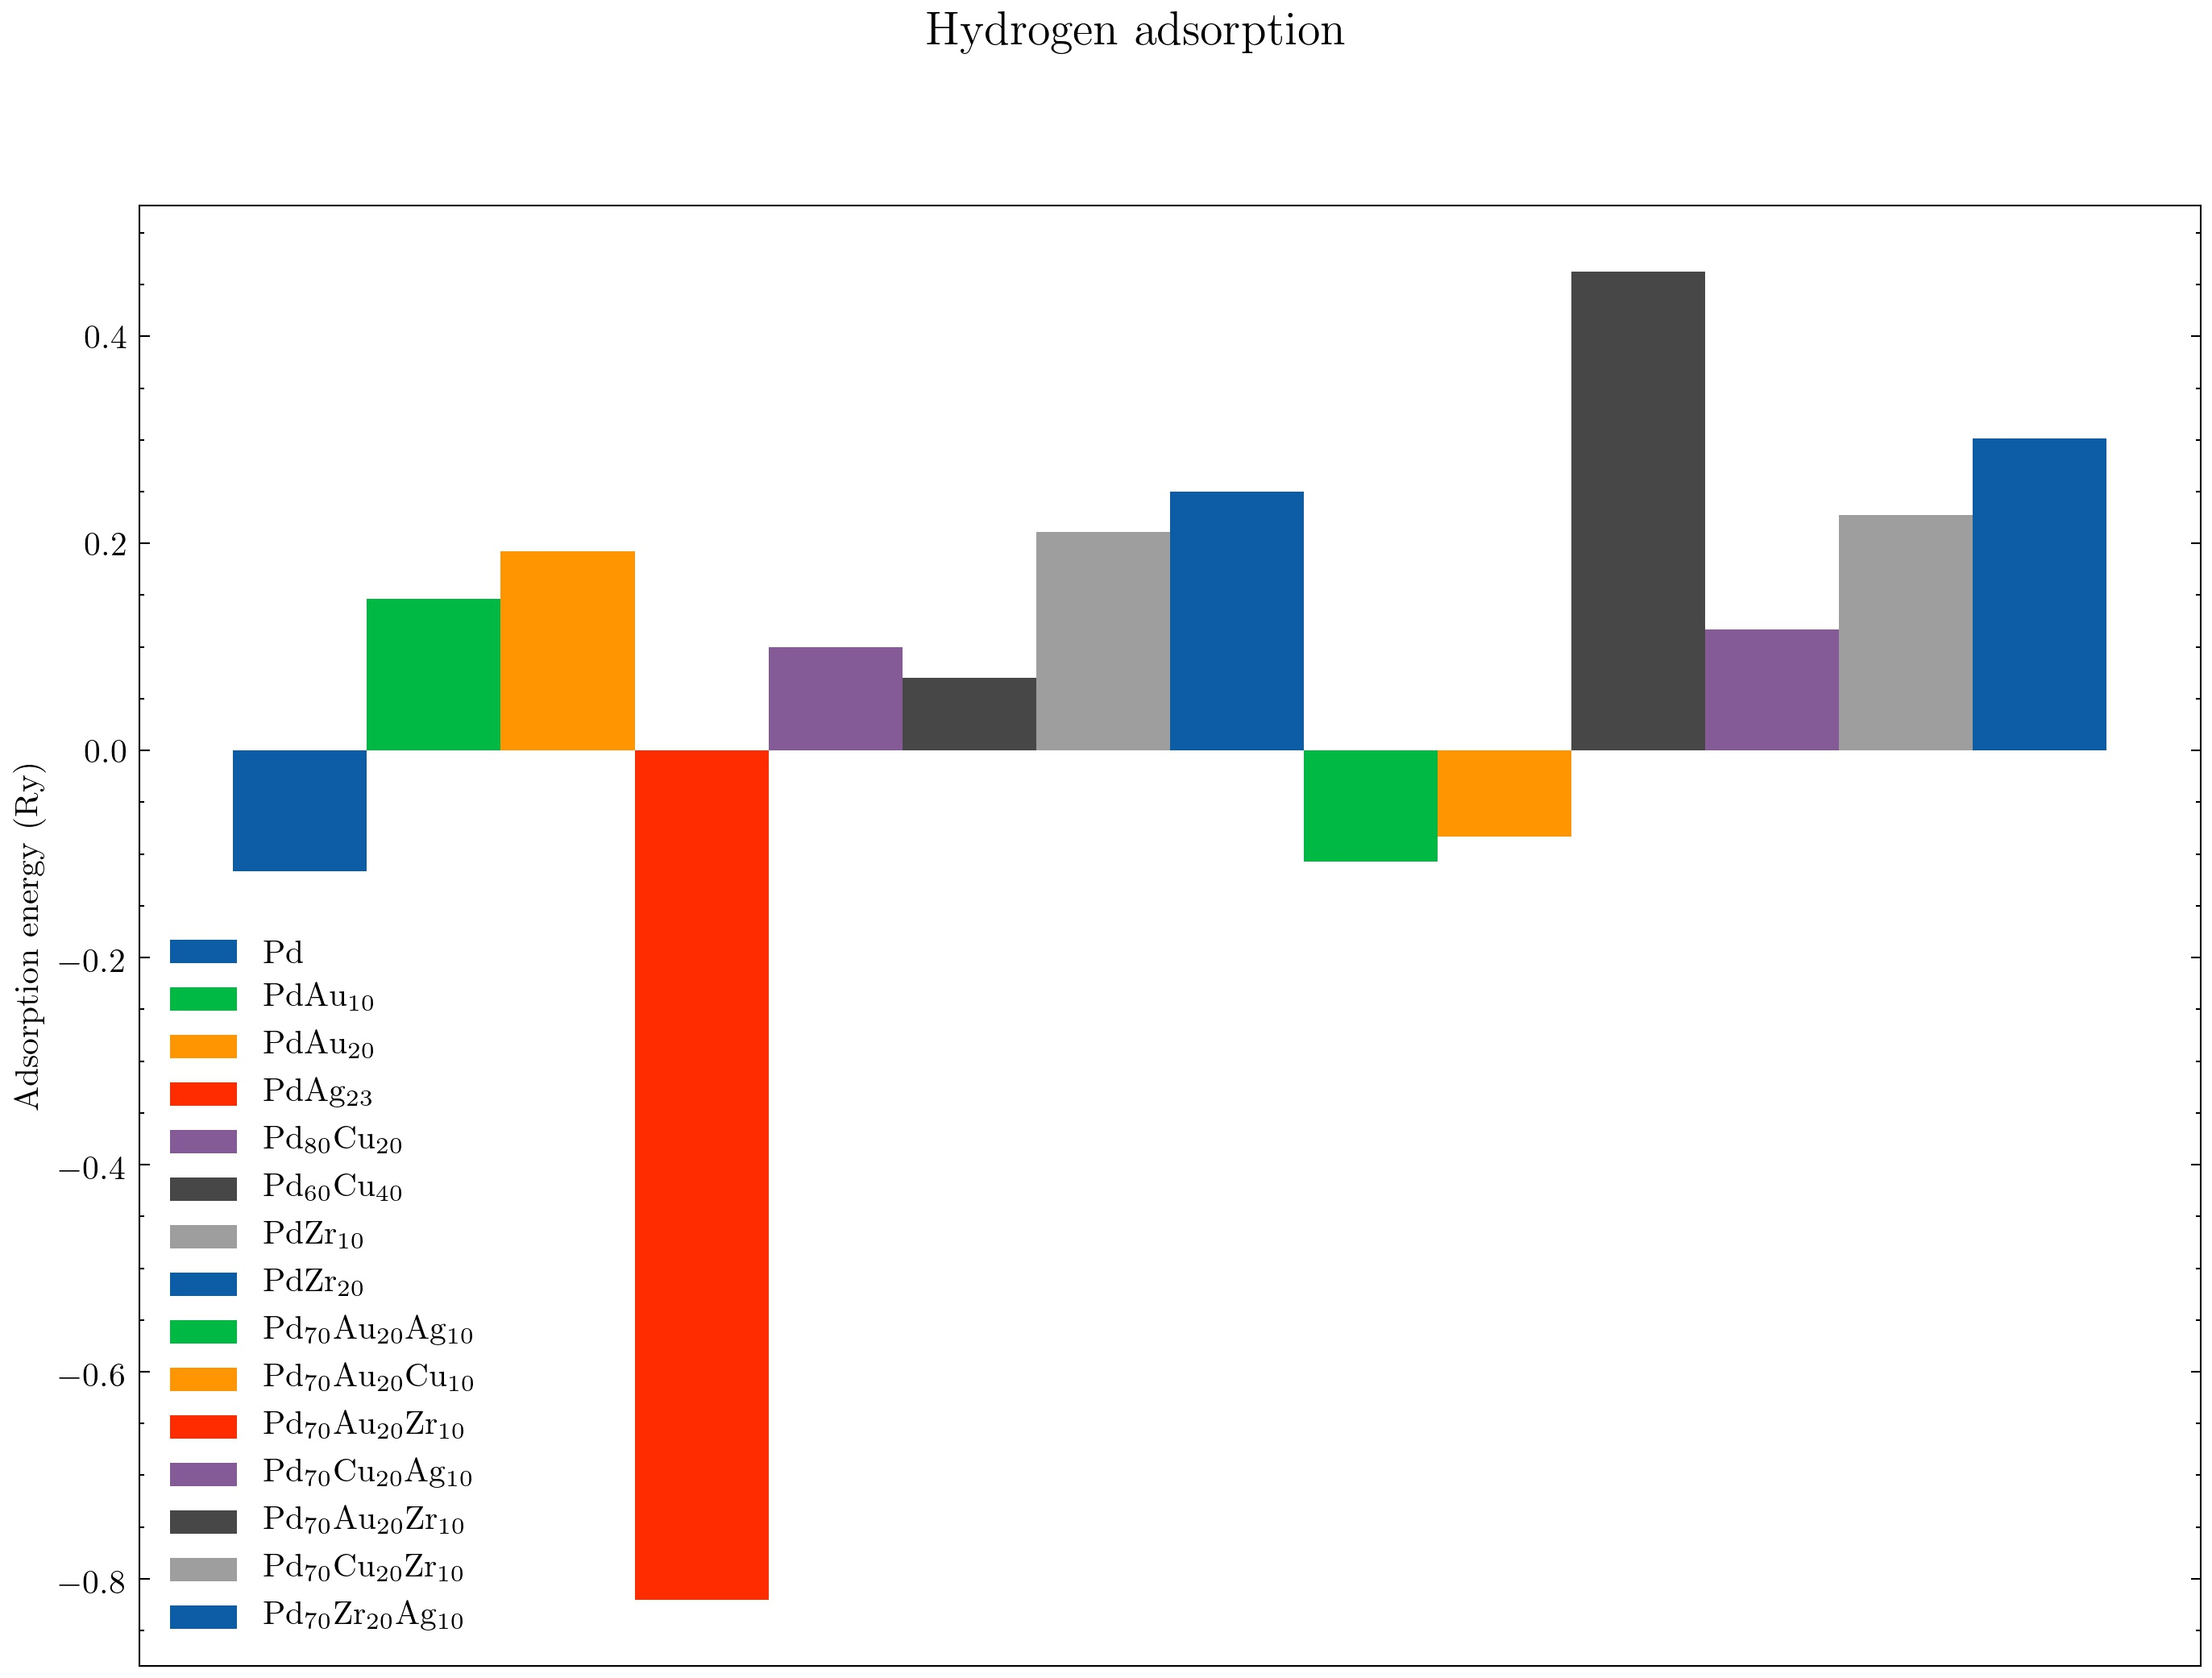
\includegraphics[width=0.9\linewidth,height=\textheight, keepaspectratio]{/Users/marc/Thesis/Chapter3/data/COads.jpg}
        \caption{Average binding energy of CO on the surface of palladium and palladium alloy slabs}
        \label{coads}
      \end{figure}
    
    \end{landscape}
\subsubsection{Ammonia}
The results of the ammonia simulations are shown in figure \ref{nh3ads}. Of the tested material compositions, neither palladium or any alloy showed an ability to readily bind with Ammonia, this was also true across all sites on the fcc and bcc lattice. This is consistent with the experimental results of Lundin et al \cite{Lundin2016} and the previous simulations by Herron et al \cite{HERRON20121670}. It should be noted that the paper by Herron \cite{HERRON20121670} found that while ammonia itself did not bind with the surface of palladium, radicals which can be created from ammonia such as imidogen (NH) and azanide (NH\textsubscript{2}) will readily form bonds. It is however extremely unlikely that these compounds wil be present in fuel cell hydrogen, and in the unlikely event they are they will likely instantly reform into the more stable NH\textsubscript{3}. It can be concluded therfore that NH\textsubscript{3} will create no challenges for the operation of palladium membranes. 

  \begin{figure}
      \centering
      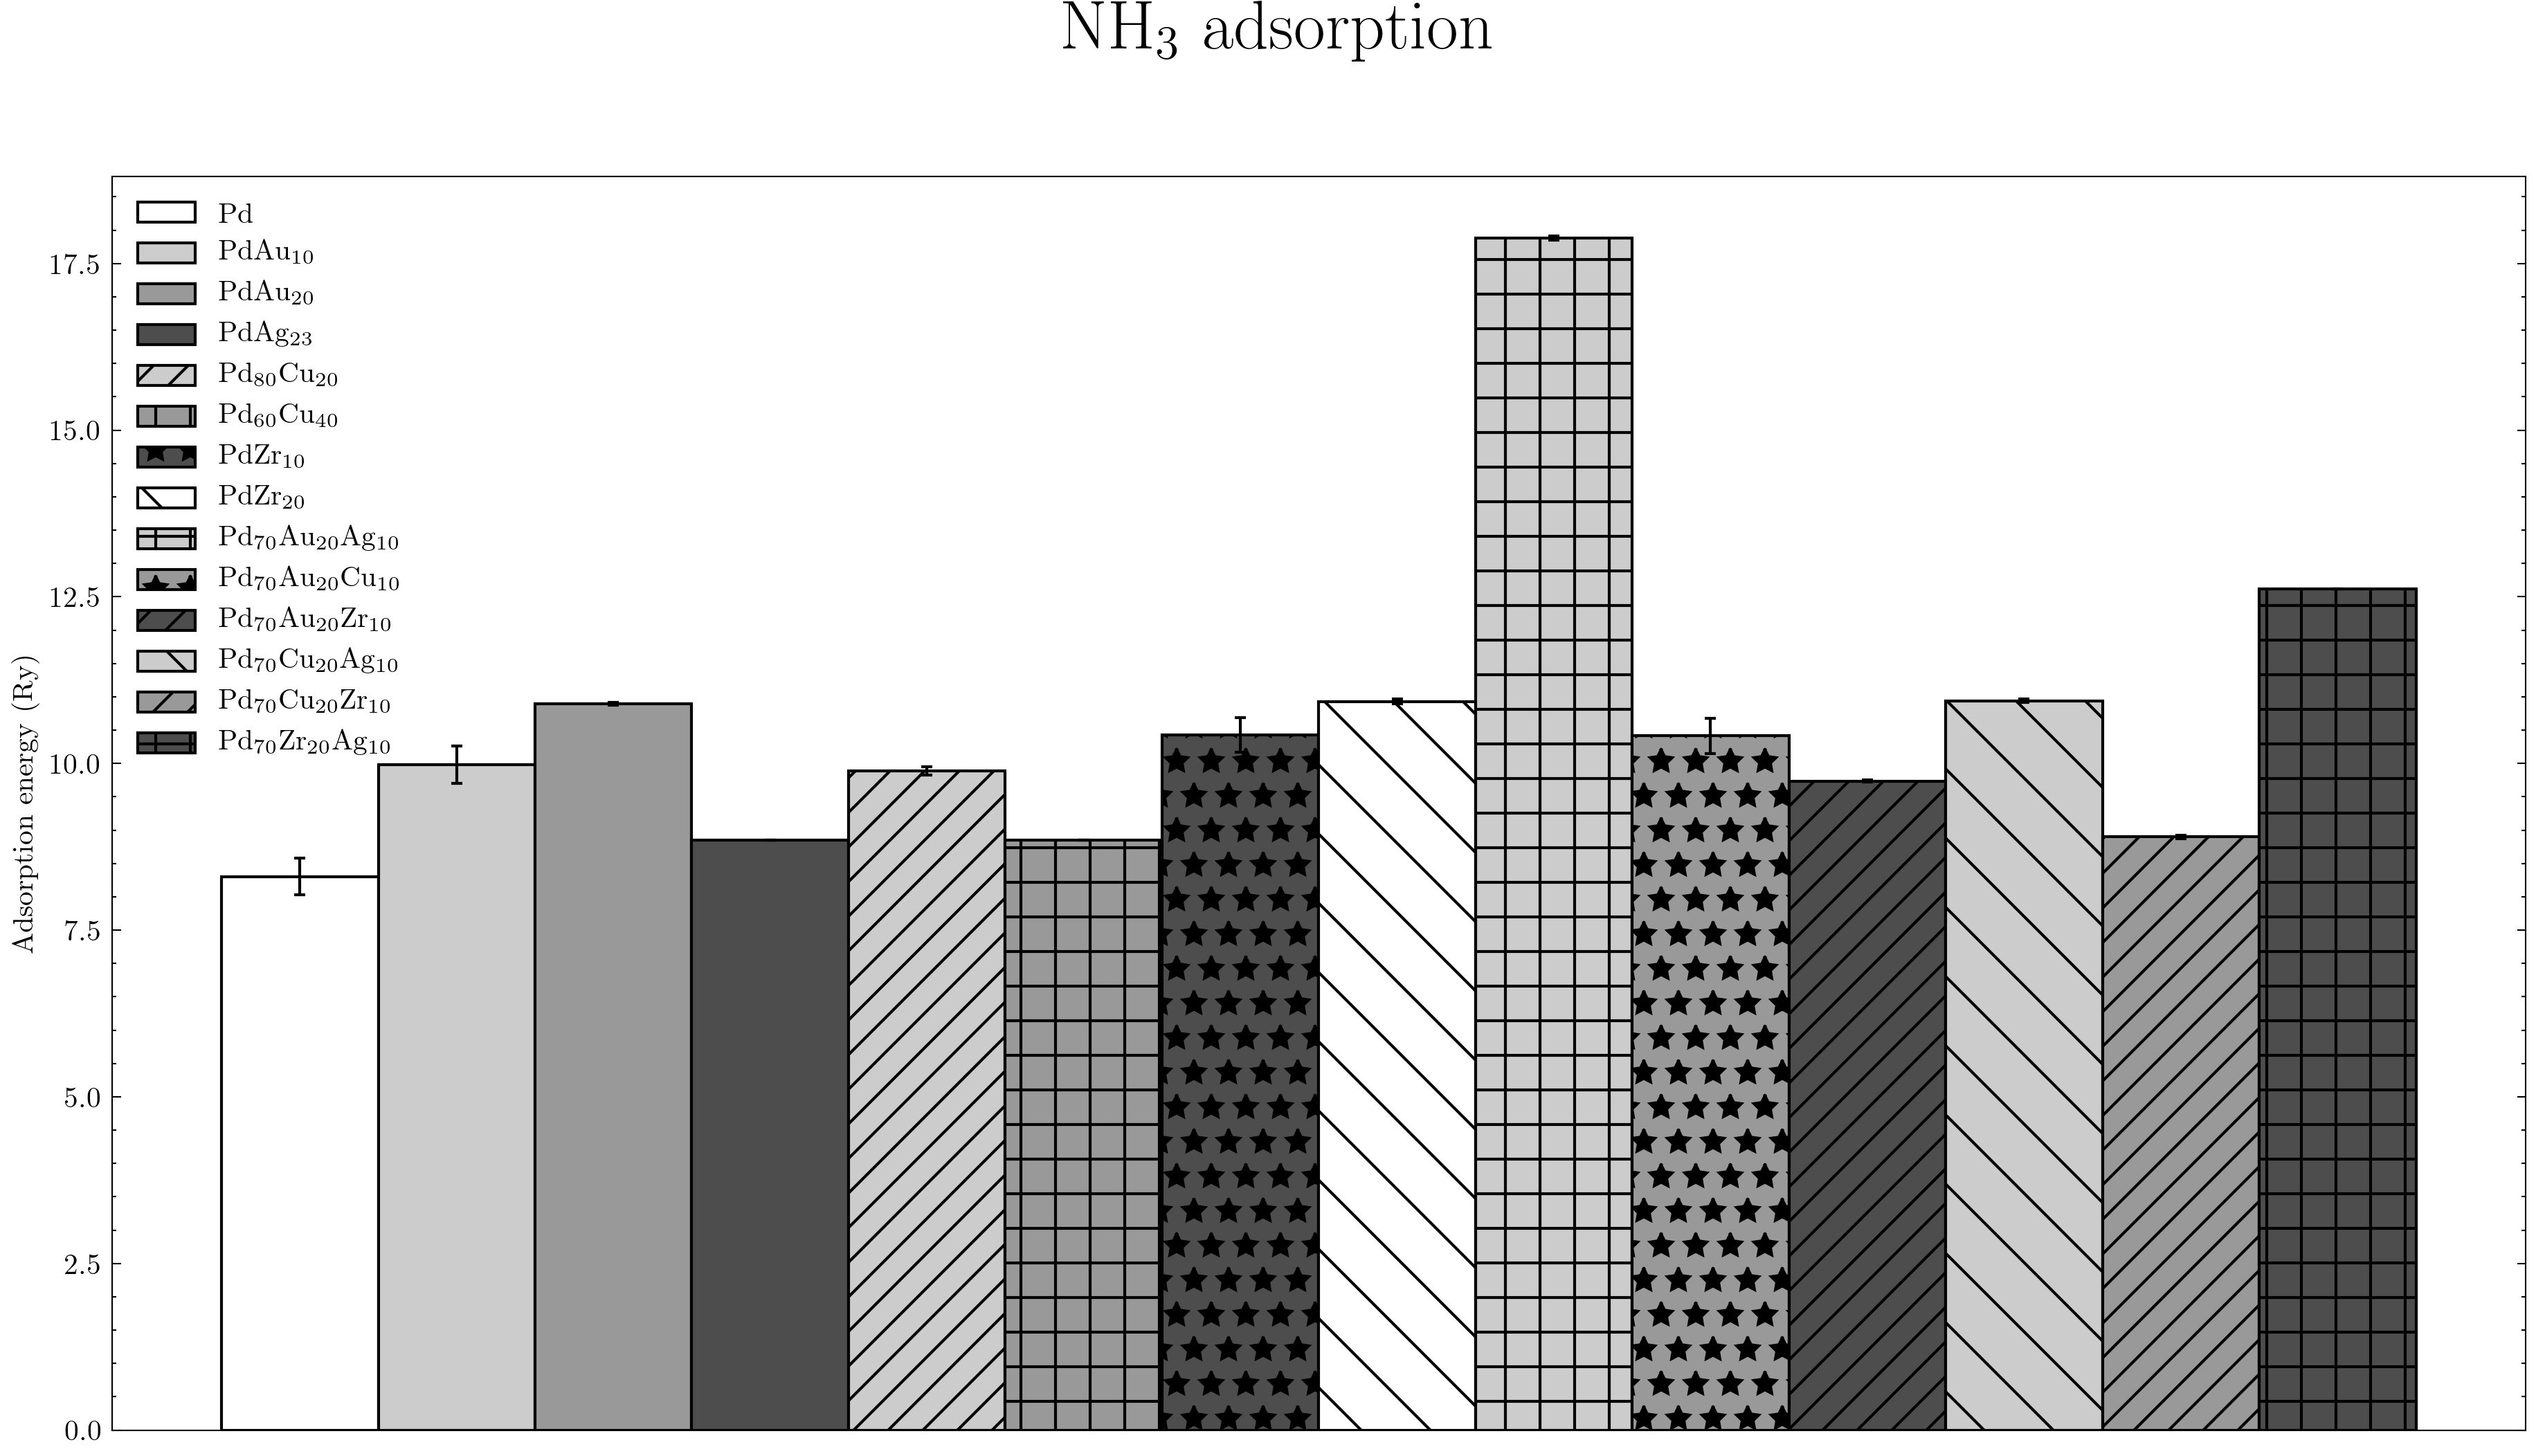
\includegraphics[width=0.9\linewidth,height=\textheight, keepaspectratio]{/Users/marc/Thesis/Chapter3/data/NH3ads.jpg}
      \caption{Average binding energy of NH\textsubscript{3} on the surface of palladium and palladium alloy slabs}
      \label{nh3ads}
    \end{figure}
  
\subsubsection{Oxygen and Water}
Since O\textsubscript{2} is a symetrical molecule binding was performed similarly to H\textsubscript{2} in section \ref{Hsection}, the results of which are shown in figure \ref{O2ads}. Alloys consisting mainly of noble metals (Pd, Ag, Au) typically did not readily bind with oxygen. Whereas alloys containing non-noble metals (Zr and Cu) showed a preference towards oxygen binding. This can pose an issue during enrichment and will likely lead to either the formation of oxides on the surface of the membrane, or catalyse a reaction between either oxygen and hydrogen, or oxygen and one of the other gaseous impurities. In the former the formation of oxides creates a shift in the lattice parameter, similar to the $\alpha - \beta$ transition seen in pure palladium membranes (figure \ref{lit-alphabeta})\cite{Li2008b} and cause membrane failure. In the latter results from hydrogen impurity can be thrown off. Therefore if oxygen is expected in the sample Zr and Cu containing alloys should be avoided.

Water adsorption was performed by attaching the O atom to each avaliable site as per previous studies. \cite{Roques2009} The results are shown in figure \ref{H2Oads} and follow the same trend as the O\textsubscript{2} results discussed above. One important caveat when considering water binding on the surface of metals is the ability for H\textsubscript{2}O molecule to form hydrogen bonds with neighbouring molecules.\cite{PhysRevB.69.195404} While this study only considered the influence of a single water molecule, in real tests the system will likely have a number of water molecules present. The effect of the hydrogen bond would likely result in the further stabilisation of future water molecules onto the surface, creating an exponential increase in adsorbed H\textsubscript{2}O. \cite{PhysRevB.69.195404} Care should also be taken, as previous studies on other metallic systems have shown that the binding of water often leads to subsequent dissociation, and formation of a metal oxide and hydrogen. Leading to the same problems with oxidation as previously discussed. \cite{doi:10.1021/jz300994e}

In conclusion noble metals appear to be the best alloying compounds to protect against the influence of H\textsubscript{2}O and O\textsubscript{2}. This is to be expected as these metals are traditionally resistant to oxidation. It should be noted however that while this study focused on binding of water on the membrane, it does not take into account adsorption on any other components and fittings on a system. Water in particular is notoriously difficult to remove from a system due to it's avaliability for binding on metal surfaces.\cite{BACQUART20205565} Therefore while reducing it's effect on the membrane solves one problem, it's effect on the overall system still has to be considered. 

\begin{landscape}
  \begin{figure}
      \centering
      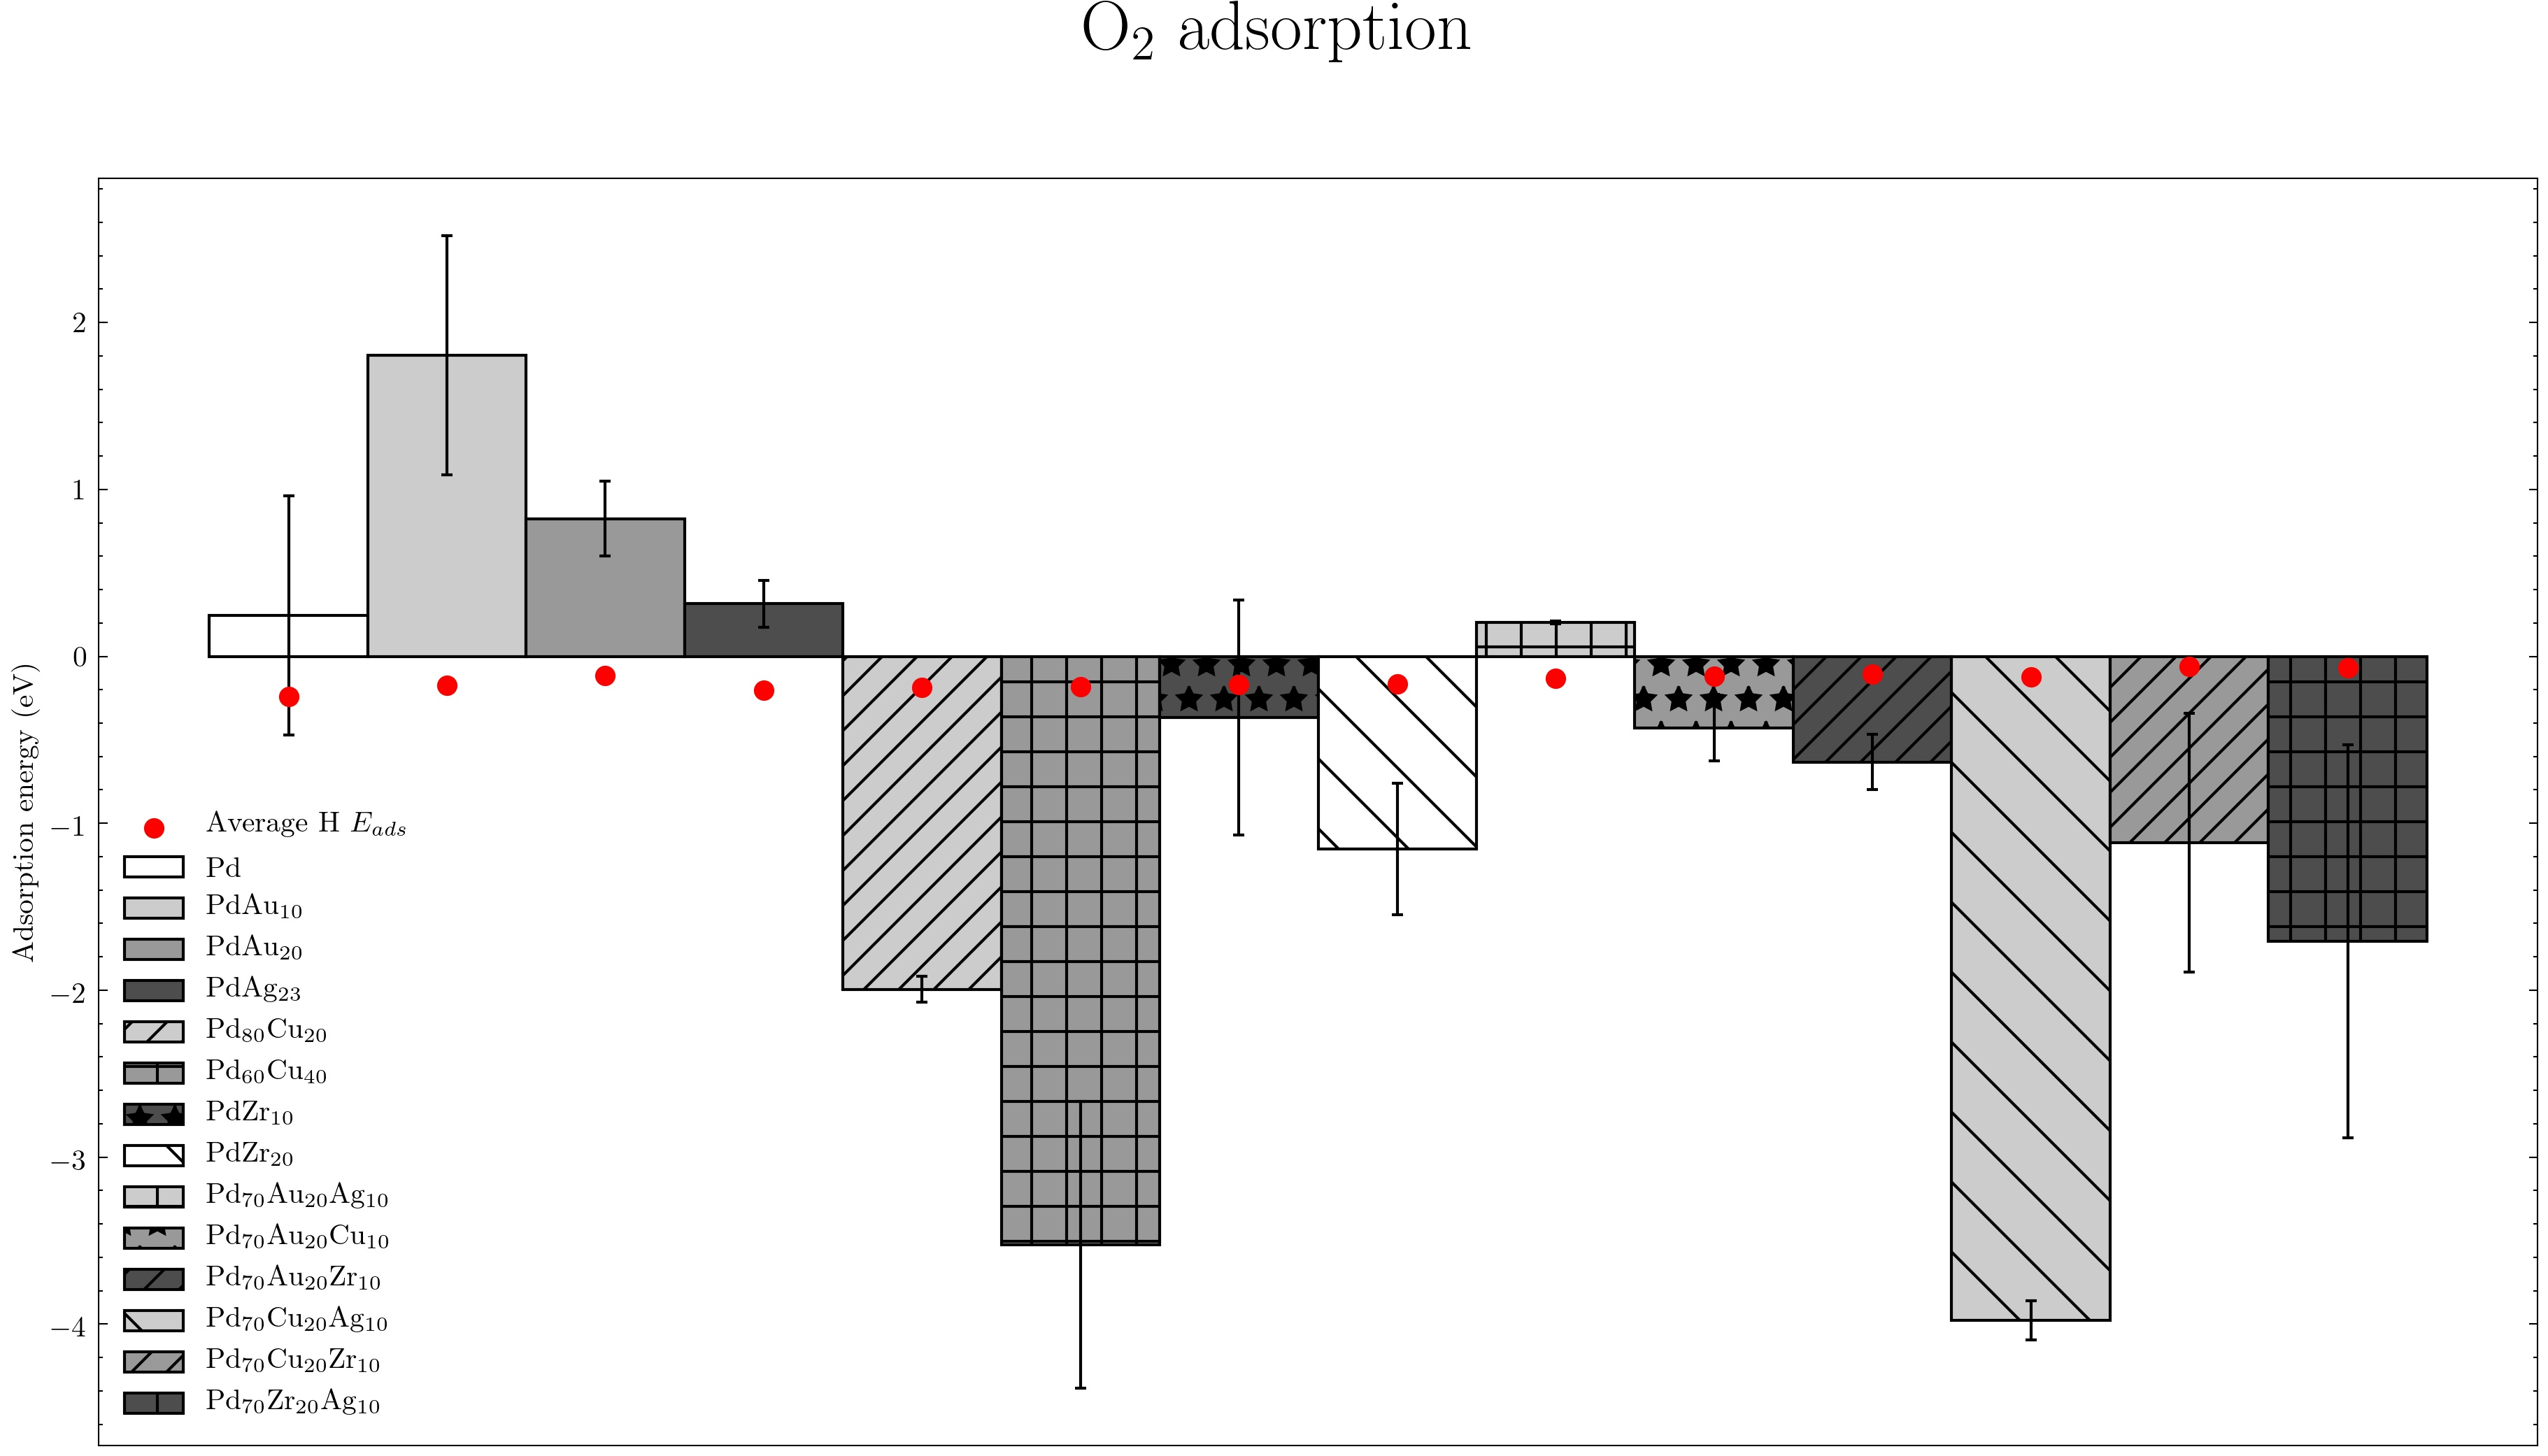
\includegraphics[width=0.9\linewidth,height=\textheight, keepaspectratio]{/Users/marc/Thesis/Chapter3/data/O2ads.jpg}
      \caption{Average binding energy of O\textsubscript{2} on the surface of palladium and palladium alloy slabs}
      \label{O2ads}
    \end{figure}
  
  \end{landscape}


\begin{landscape}
  \begin{figure}
      \centering
      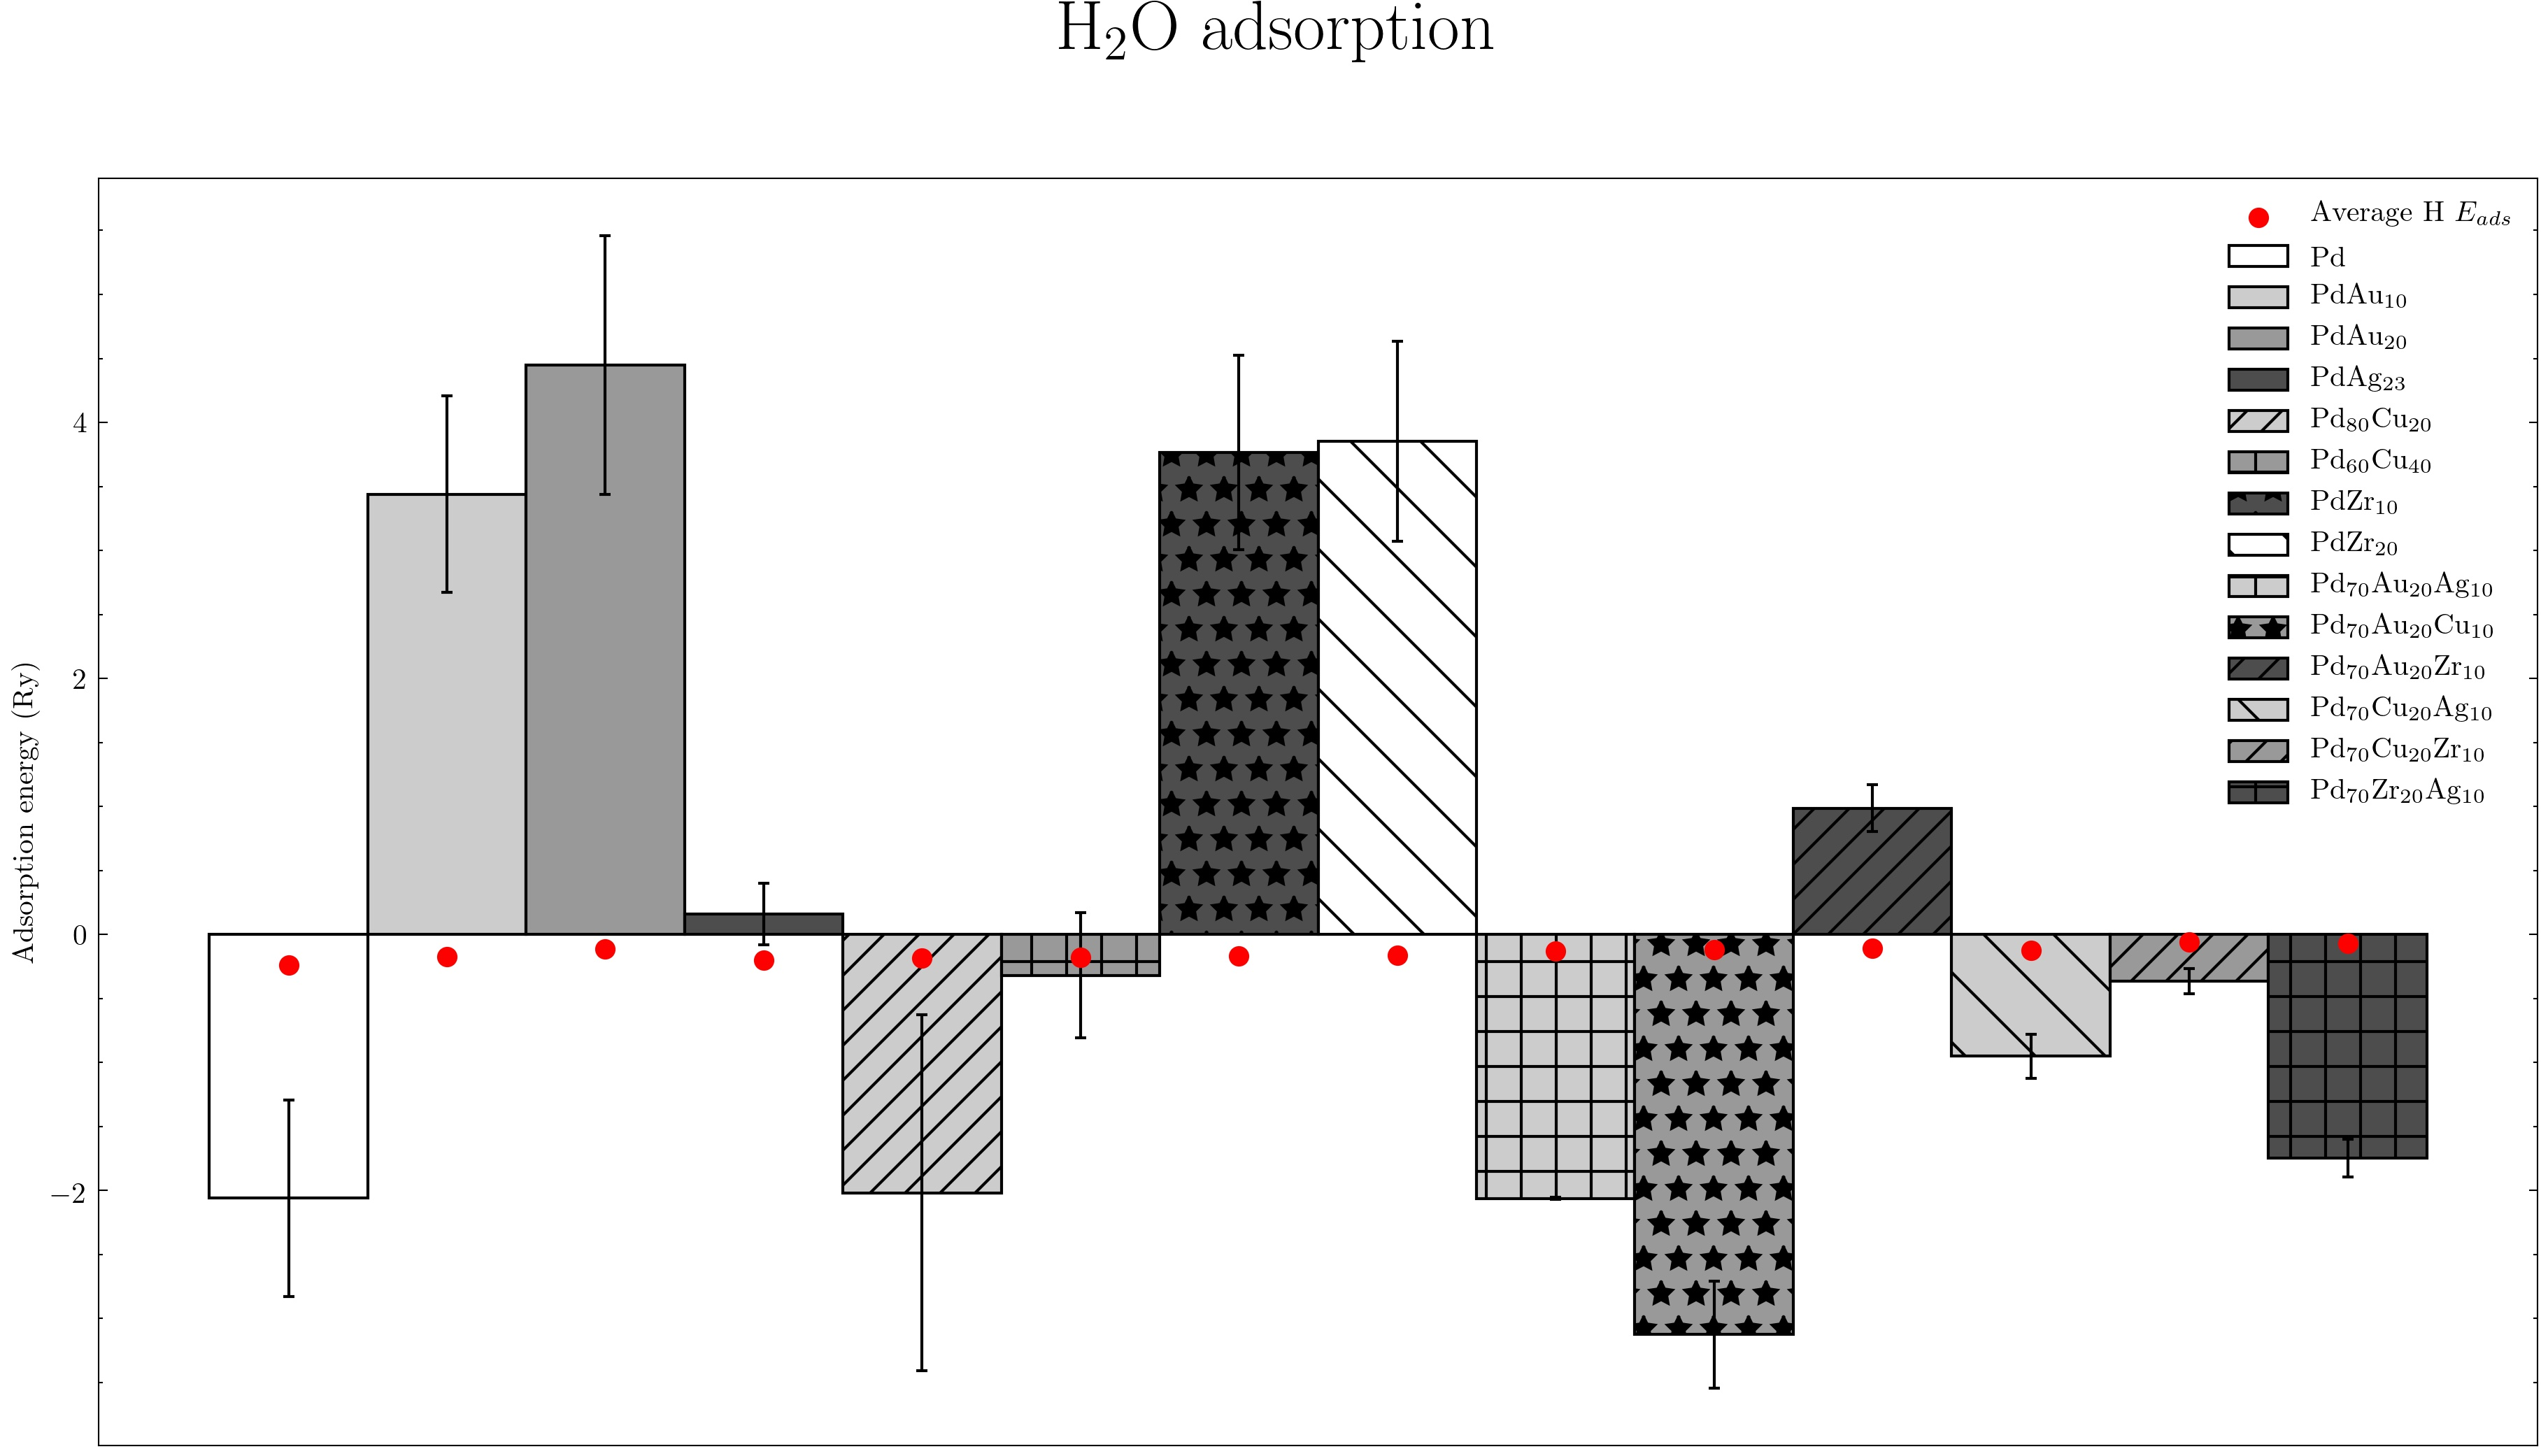
\includegraphics[width=0.9\linewidth,height=\textheight, keepaspectratio]{/Users/marc/Thesis/Chapter3/data/H2Oads.jpg}
      \caption{Average binding energy of H\textsubscript{2}O on the surface of palladium and palladium alloy slabs}
      \label{H2Oads}
    \end{figure}
  
  \end{landscape}

\subsubsection{Methane}

Methane was adsorbed onto the surface of the Pd slab systems using one of the hydrogen molecules as has previously been performed in literature. \cite{doi:10.1021/acsomega.8b02578} The results of the simulations are shown in figure \ref{CH4ads}. 

All simulated metals seem to have the ability to bind CH\textsubscript{4} to its surface. Intuitivley this seems reasonable since the atom binding to the surface is H\textsubscript{2}, which we have already proven has the ability to bind to all Pd alloy models. The molecule also features a carbon molecule which from our CO simulations in figure \ref{coads} will also preferentially bind to the surface of the Pd slab models, at a higher preference than hydrogen. The results of the CH\textsubscript{4} simulations seem to follow the general trend of it's sister CO results, however at a weaker level.  All simulations were unstable which is shown by the large error values showing large swings in the results from each simulation. Therefore it is likely that in many simulations, while CH\textsubscript{4} is stable on the surface, could not find the most stable coordination due to competing forces acting from the hydrogen atoms, and the carbon atom. 

The binding energies of CH\textsubscript{4} on each site in the Pd system are shown in figure \ref{CH4site}. Similarly to CO, the CH\textsubscript{4} molecule has a higher preference to the FCC and HCP sites than H. Unlike CO, CH\textsubscript{4} does not bind as strongly to the TOP site as CO. The reason for the strong binding preference to the FCC and HCP sites is likely due to the fact that while the H atom is bound within the HCP and FCC sites, the C atom and other H atoms will bind to the surrounding metallic atoms in the crystalline lattice, stabilising the molecule in those sites. On the TOP and BRIDGE sites this does not happen, and since the H atom is bound more strongly to C through a covalent bond, the resulting energy avaliable for binding on these sites is lower than it would be if the molecule was pure hydrogen. 

In terms of resistence to CH\textsubscript{4} binding, the conclusions reached in the section discussing the results of CO still hold true. All alloy compositions with high percentages of Au and Ag showed higher resistance to CH\textsubscript{4} binding, whereas Cu and Zr containing molecules performed worse. 

Past studies performing CH\textsubscript{4} binding on metallic surfaces found that in some cases the H atom could dissociate from the molecule, creating CH\textsubscript{3} and H. \cite{doi:10.1021/acs.jpcc.8b03184} In this particular application such a reaction would result in the liberated H atom permeating through the membrane, leaving CH\textsubscript{3} on the retentate side. While this changes the composition of the retentate gas, from a measurement perspective it should not pose much of an issue. The ISO 14687-2\cite{InternationalStandardISO14687-2:20122012} standard specifies a total hydrocarbon level and therefore any CH\textsubscript{3} that is produced should be detected using previously outlined techniques. \cite{Murugan2015}

What may pose a larger issue is that in the study performed by Herron \cite{HERRON20121670}, it was found that similar to Ammonia, CH\textsubscript{4} based radicals will bind more strongly to the surface than CH\textsubscript{4} resulting in an increasing poisoning effect. It is unknown whether the hydrogen dissociation effect previously discussed would continue to occur with these radicals, but in the case it does, the result would eventually be carbon deposition on the surface of the membrane. Eventually deactivating the membrane entirely, and throwing off all results due to removal of carbon from the gas.  

\begin{figure}
  \centering
  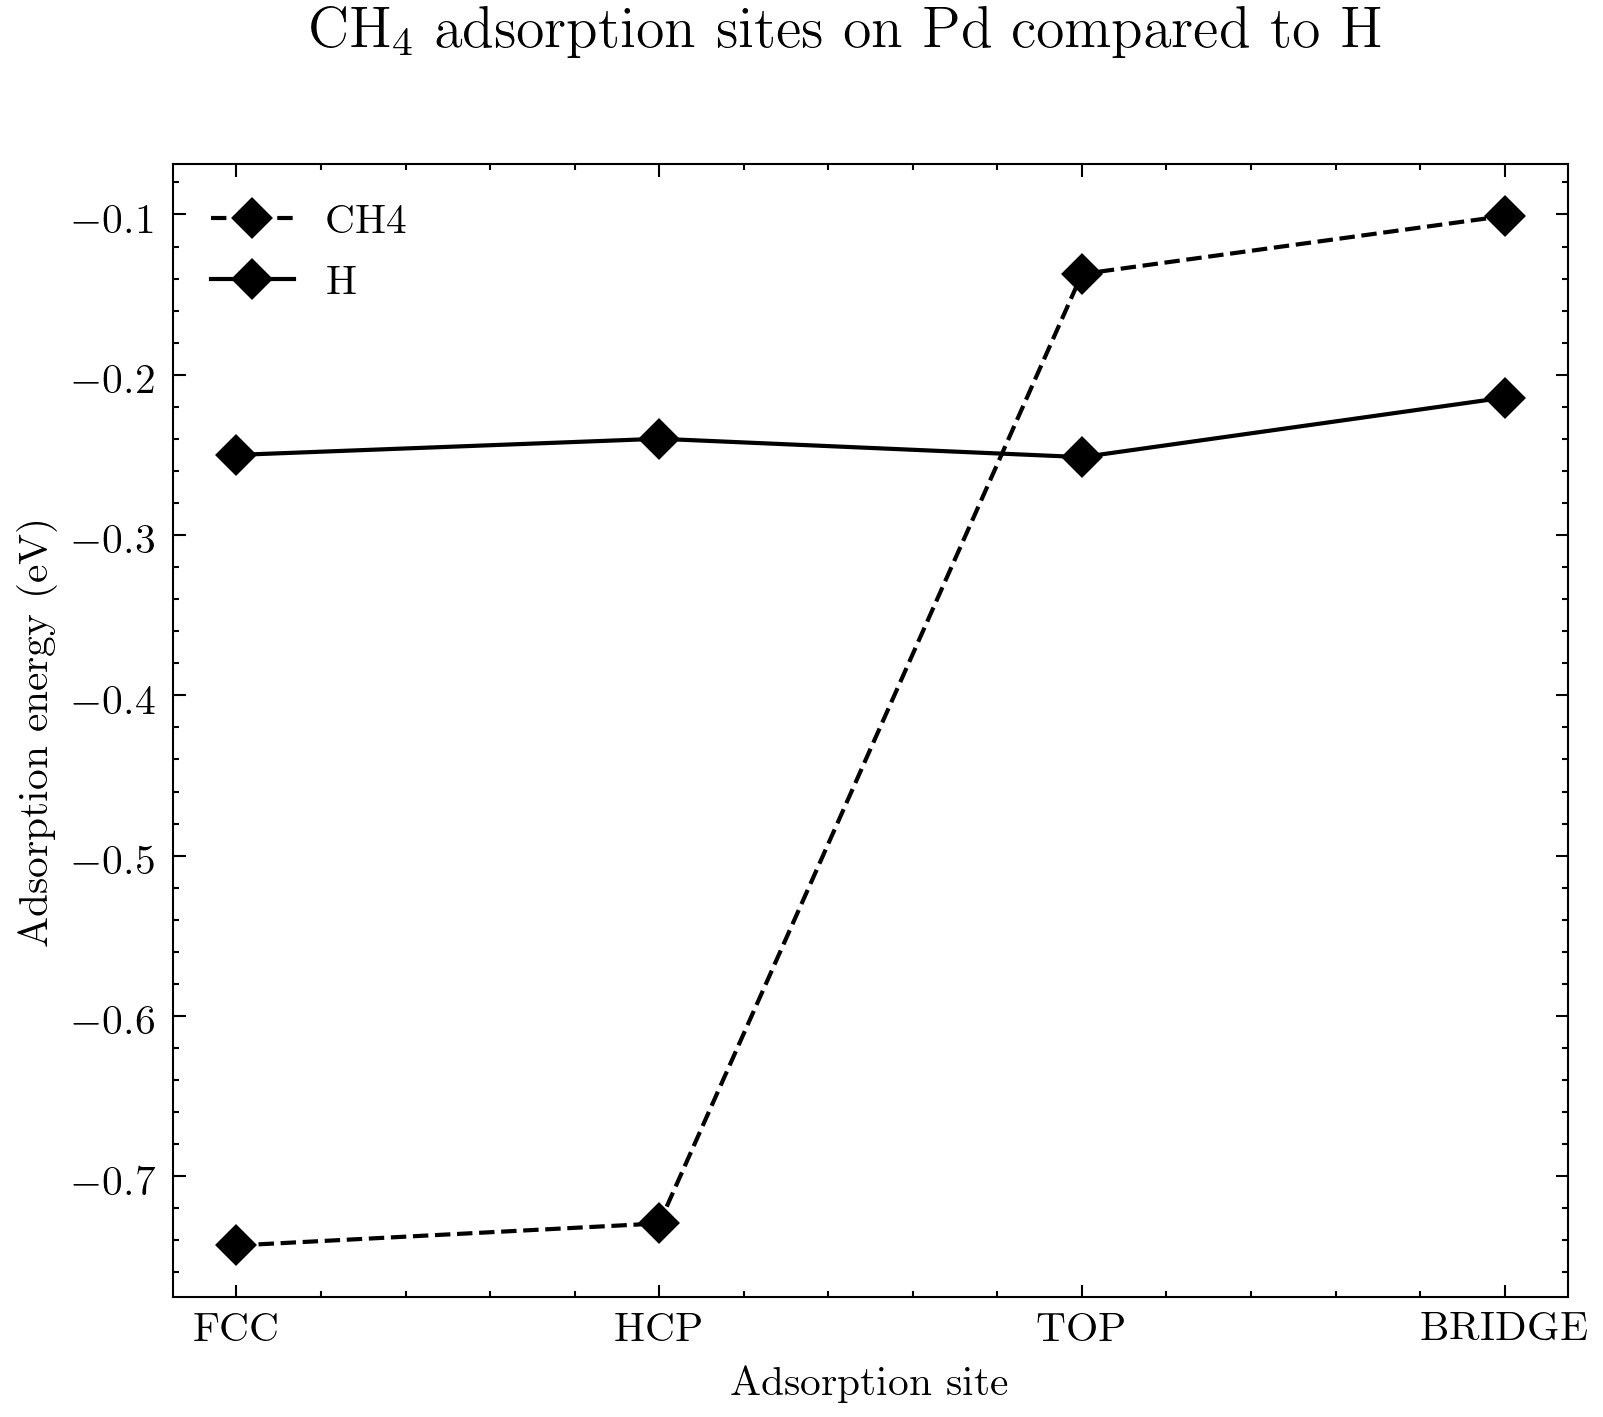
\includegraphics{/Users/marc/Thesis/Chapter3/data/CH4Sites.jpg}
  \caption{binding energy of H and CH\textsubscript{4} for each site on a 2x2x5 Pd slab}
  \label{CH4site}
\end{figure}

\begin{landscape}
  \begin{figure}
      \centering
      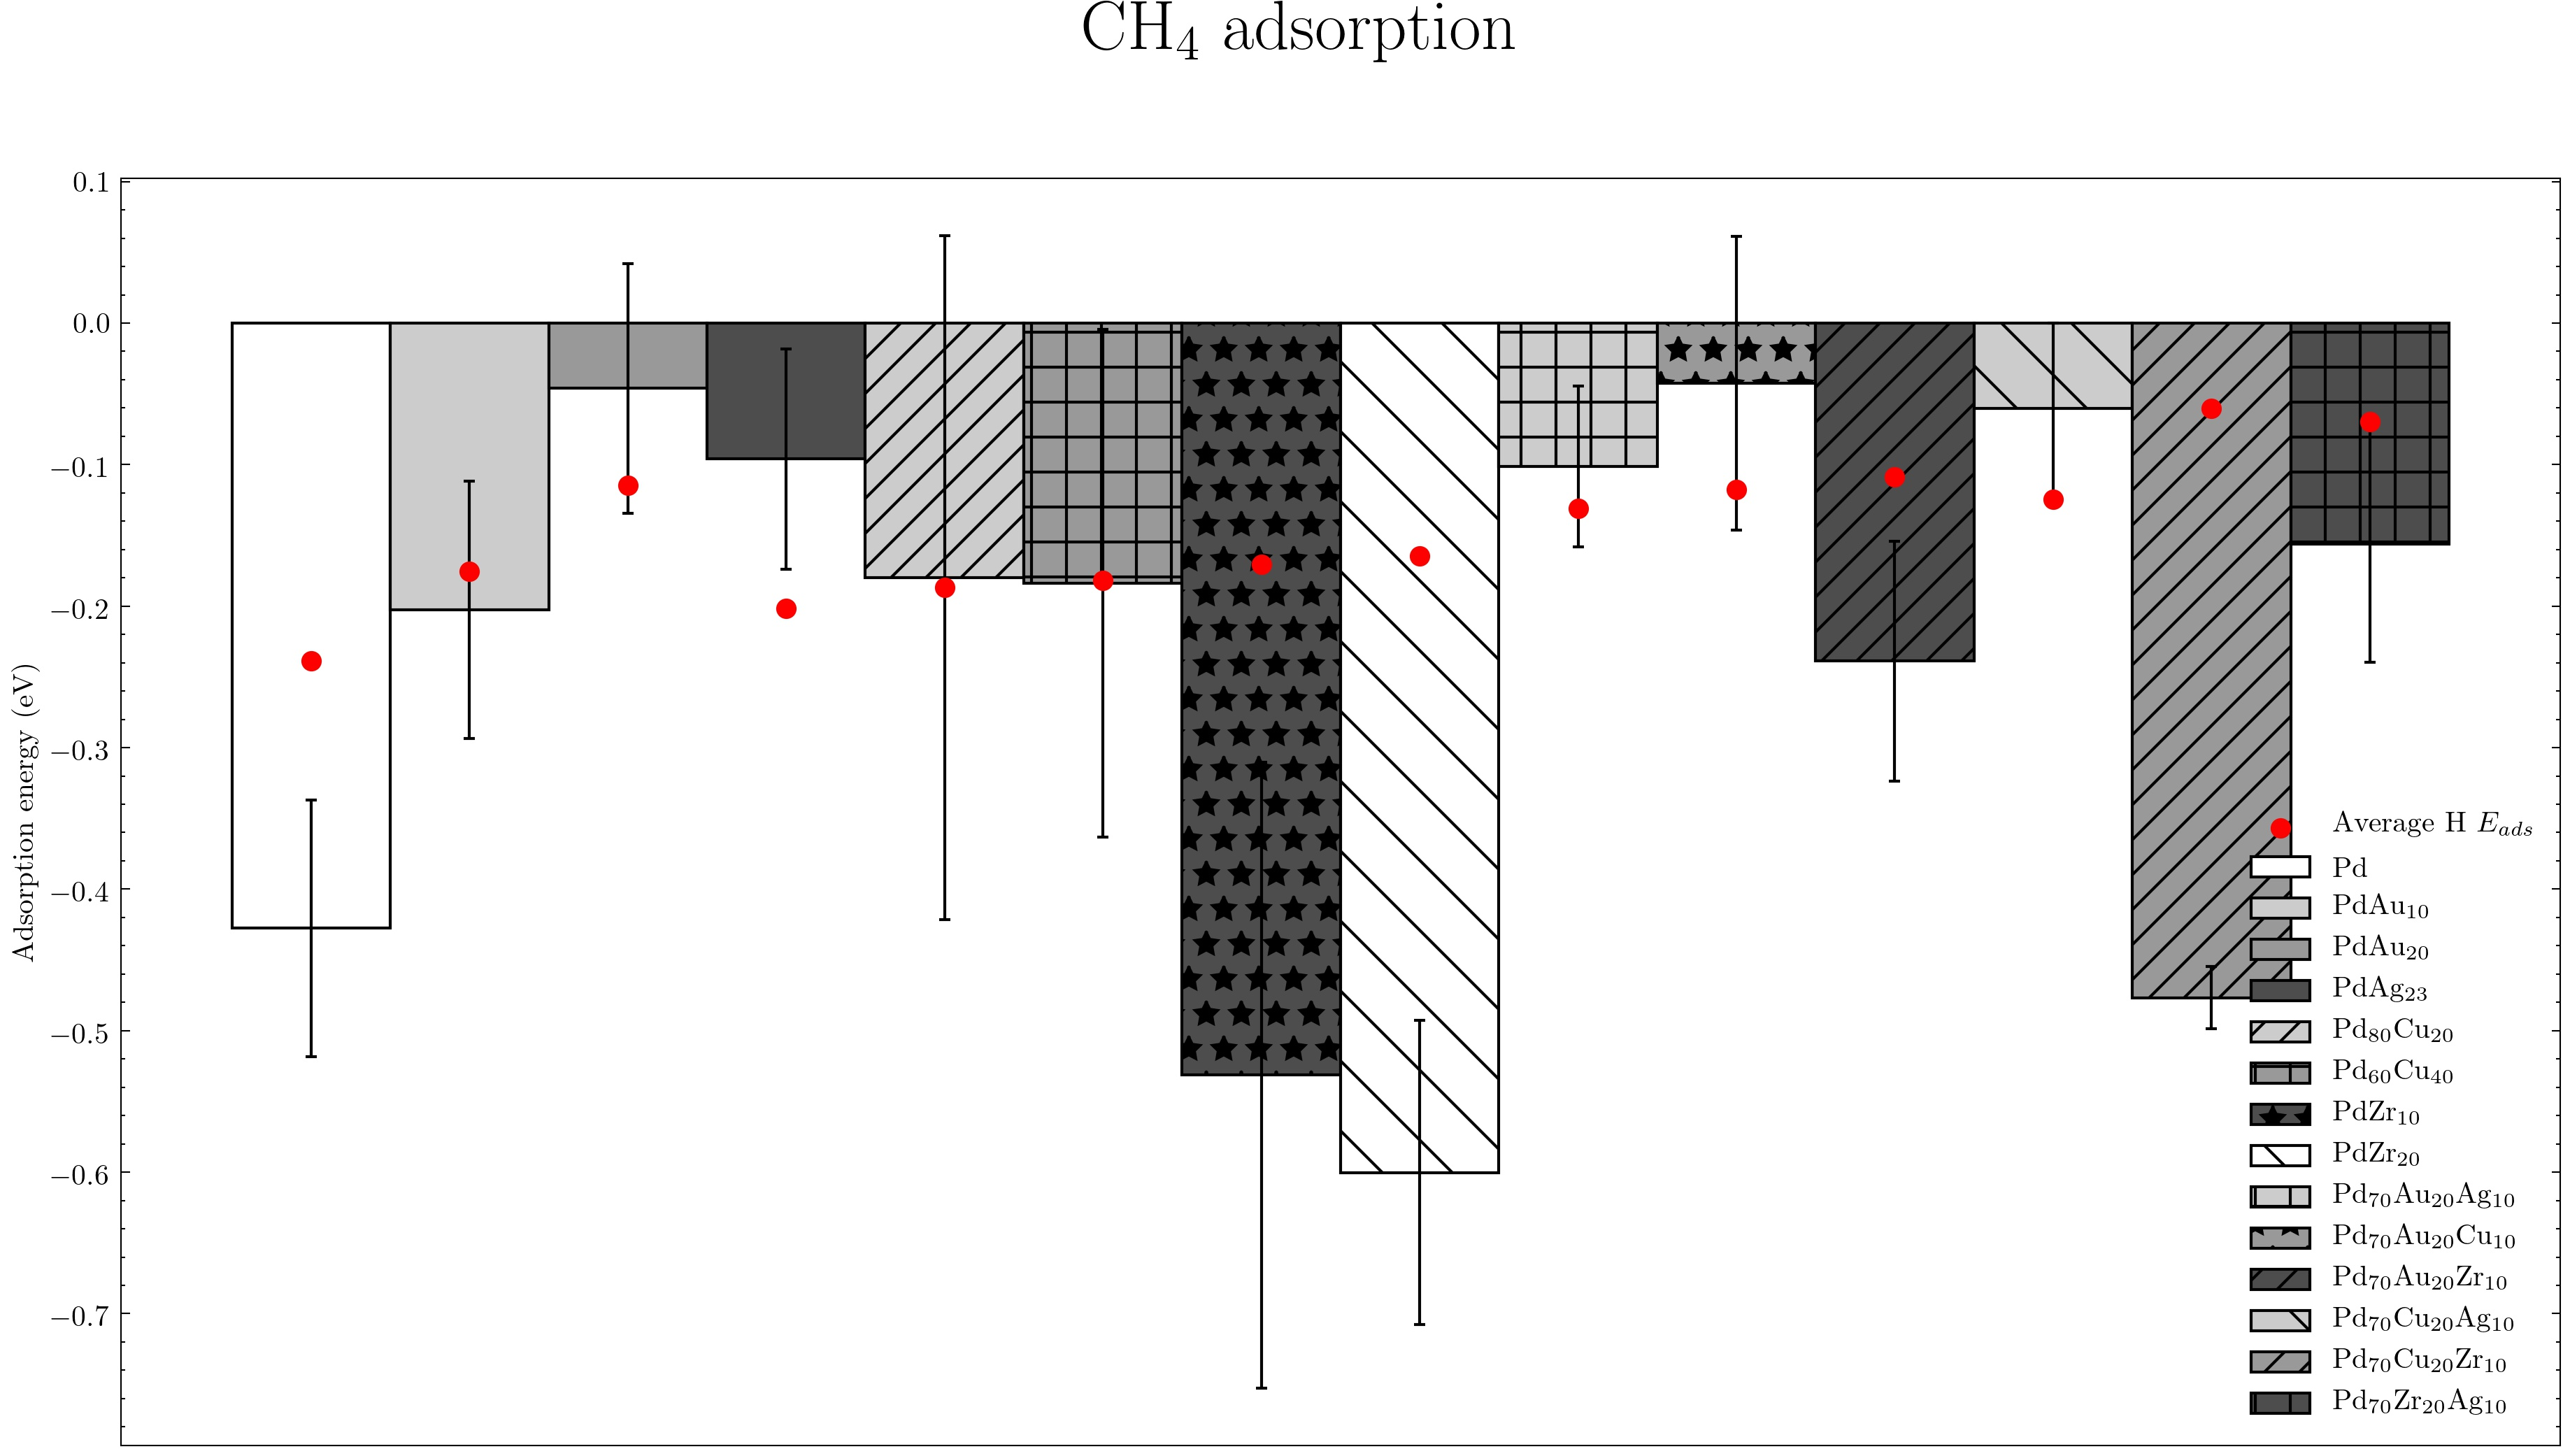
\includegraphics[width=0.9\linewidth,height=\textheight, keepaspectratio]{/Users/marc/Thesis/Chapter3/data/CH4ads.jpg}
      \caption{Average binding energy of Methane on the surface of palladium and palladium alloy slabs}
      \label{CH4ads}
    \end{figure}
  
  \end{landscape}
\subsubsection{Formaldehyde and Formic acid}

Formaldehyde and Formic acid are similar molecules, with the only different being one of the hydrogen atoms being replaced with an OH group on formic acid. Both molecules were adsorbed onto the surface using the double bonded O atom perpendicular to the surface of the slab model.\cite{C8RA04983A} The results for the simulations are shown in both figure \ref{formaldehydeads} for formaldehyde and figure \ref{FAads} for formic acid. 

The results of these simulations vary widely, with formaldehyde showing strong binding ability with Pd and Pd alloy surfaces, while Formic acid appears to reject binding completely. The systems were also largely unstable as indicated by the large error values, which indicates that there are a number of forces acting on each atom on the molecule and therefore multiple stable arrangements other than the one chosen.

This result for formaldehyde is not surpring as formaldehyde is widely known to be effective catalyst for oxidation of formaldehyde, being able to oxidise formaldehyde under the presence of sunlight alone. \cite{C6CY00062B} Therefore it is likely that any mixture containing both formaldehyde and oxygen under the presence of a palladium membrane will likely react, forming carbon dioxide and hydrogen. Additionally palladium alone may be powerful enough to dissociate the formaldehyde molecule, and depending on the coordination of the molecule form H\textsubscript{2} and CO, or hydrocarbon compounds ranging from CH\textsubscript{2} to \textsubscript{4} and oxygen,\cite{C8RA04983A} the ramifications of which have been discussed previously. Unfortunately out of the tested alloys there does not appear to be a solution to this and further membrane compositions should be screened in order to determine an appropriate material to supress the effect of formaldehyde.

Past research evaluating Pd surfaces for formic acid oxidation found that Pd surfaces typically reject COH bindings which lines up well with these results. \cite{CAPON1973239}




\begin{landscape}
  \begin{figure}
      \centering
      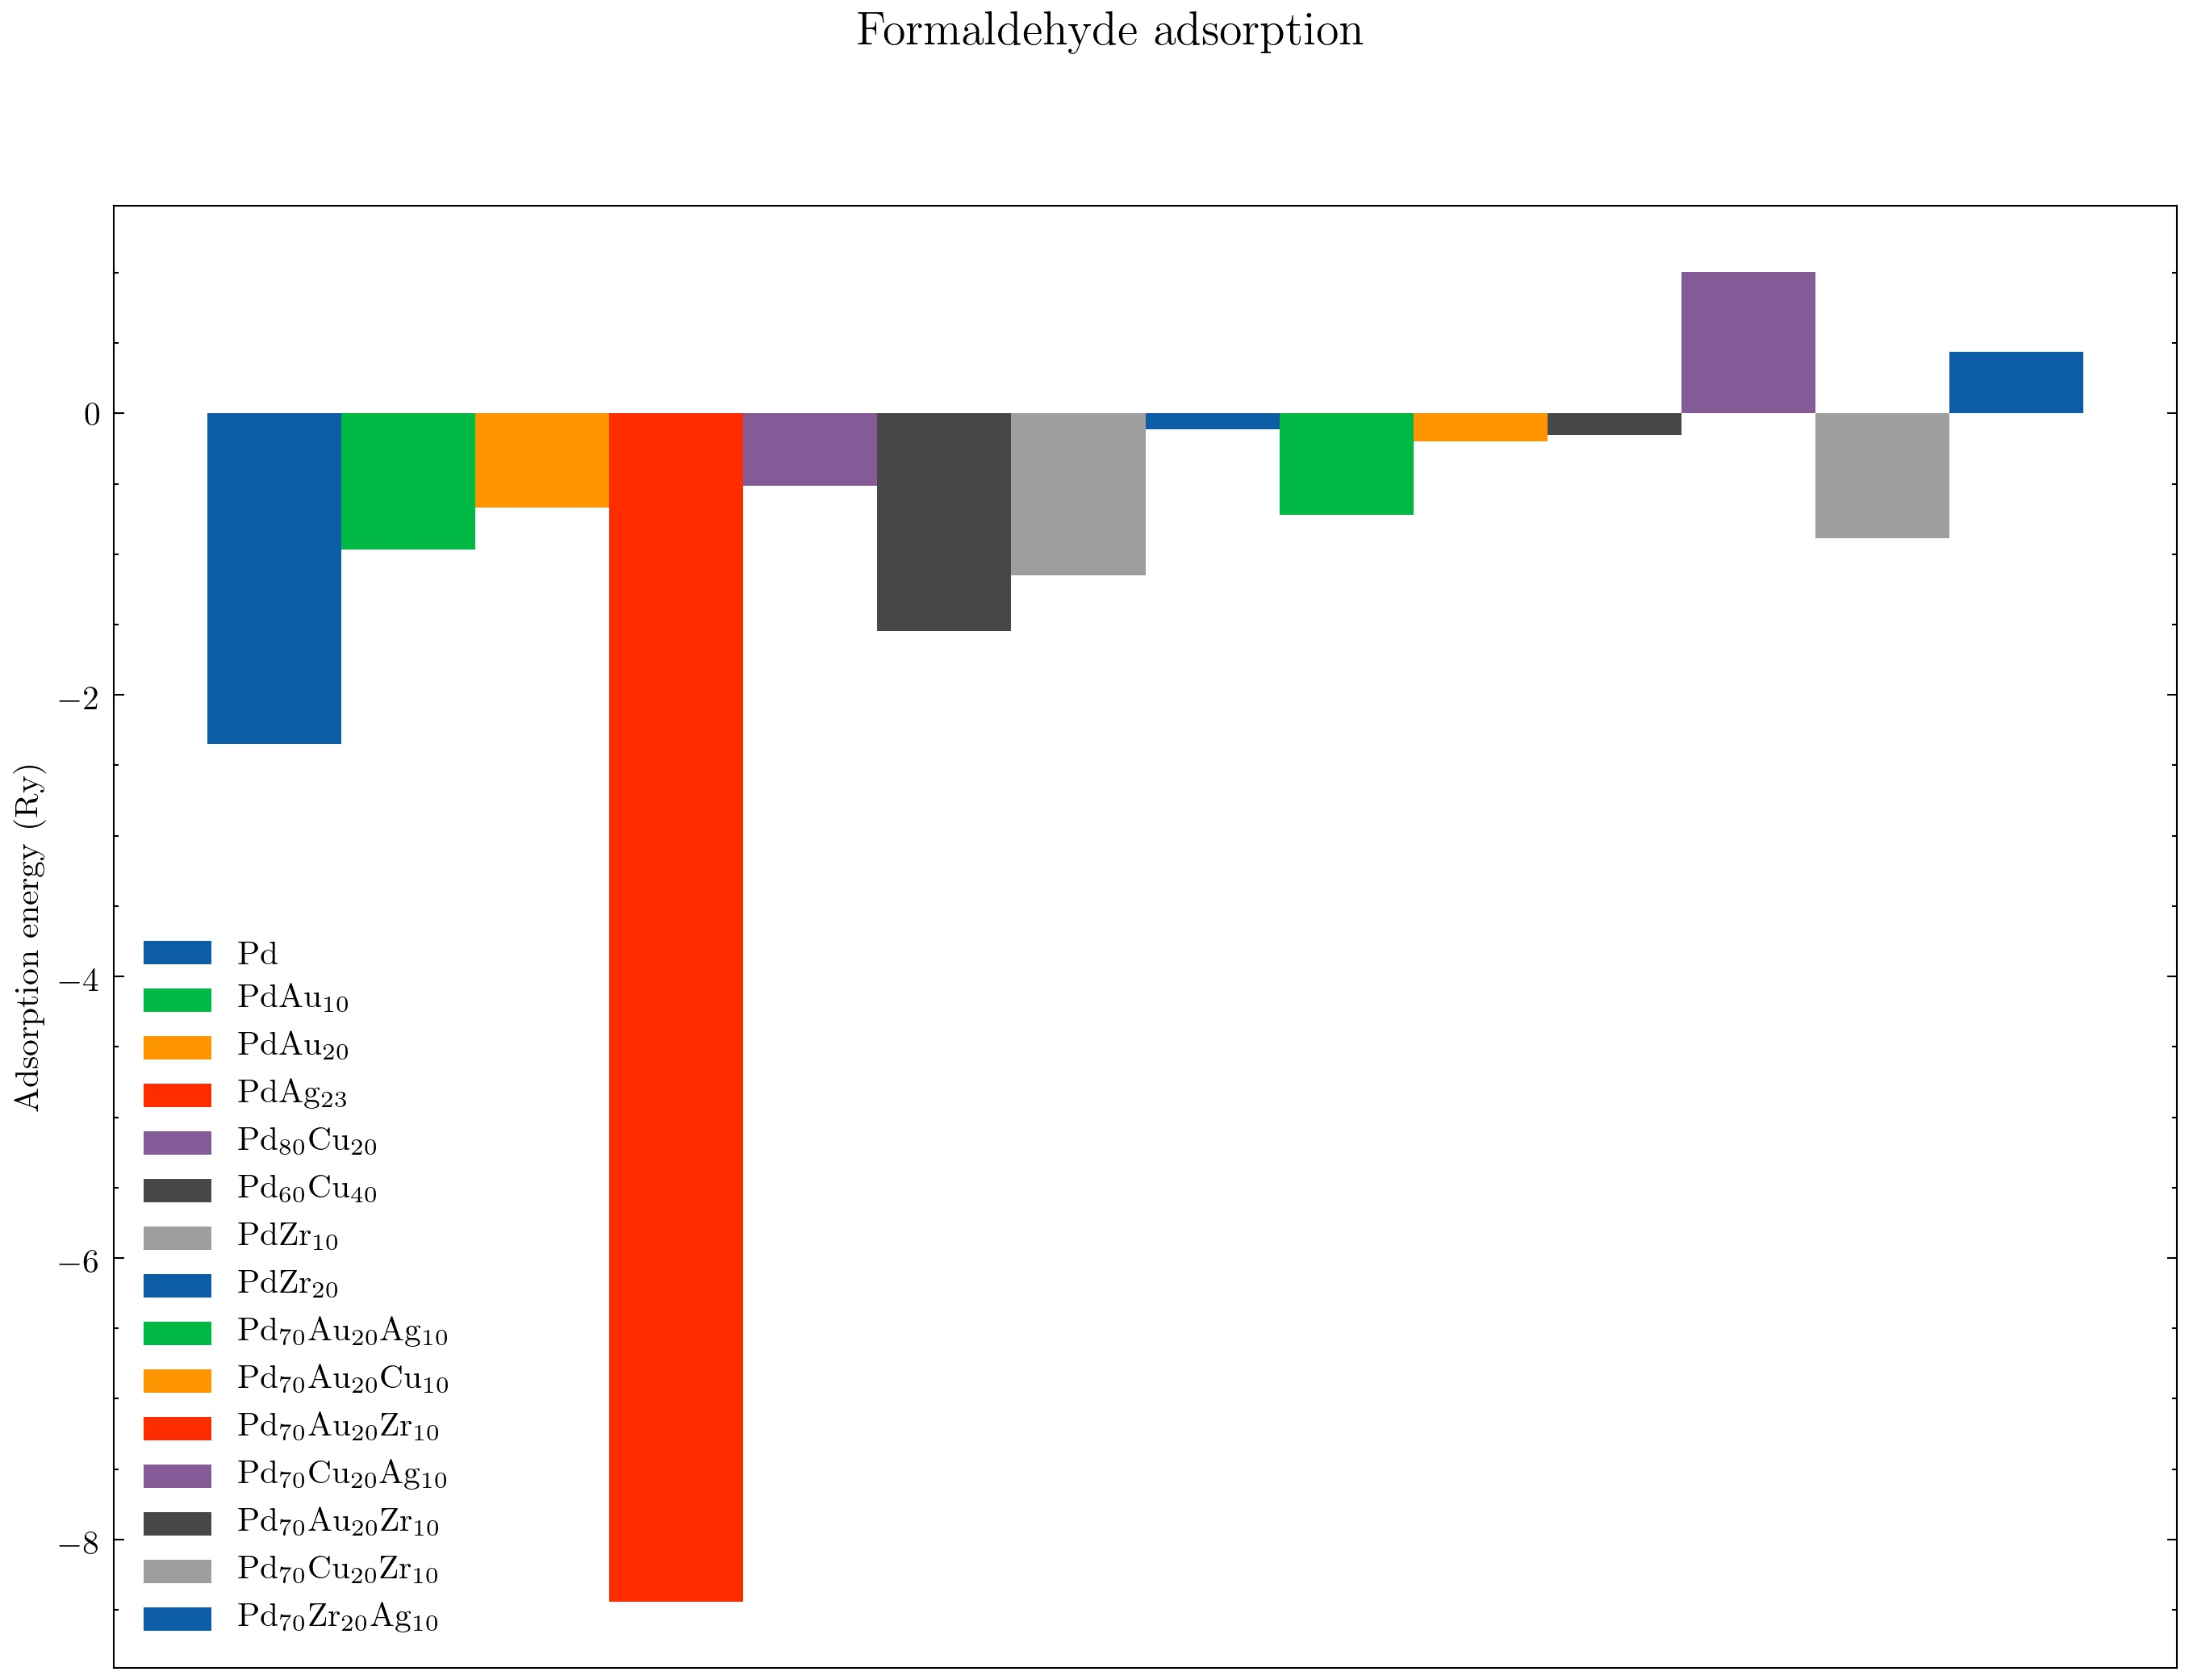
\includegraphics[width=0.9\linewidth,height=\textheight, keepaspectratio]{/Users/marc/Thesis/Chapter3/data/Formaldehydeads.jpg}
      \caption{Average binding energy of formaldehyde on the surface of palladium and palladium alloy slabs}
      \label{formaldehydeads}
    \end{figure}
  
  \end{landscape}

\begin{landscape}
  \begin{figure}
      \centering
      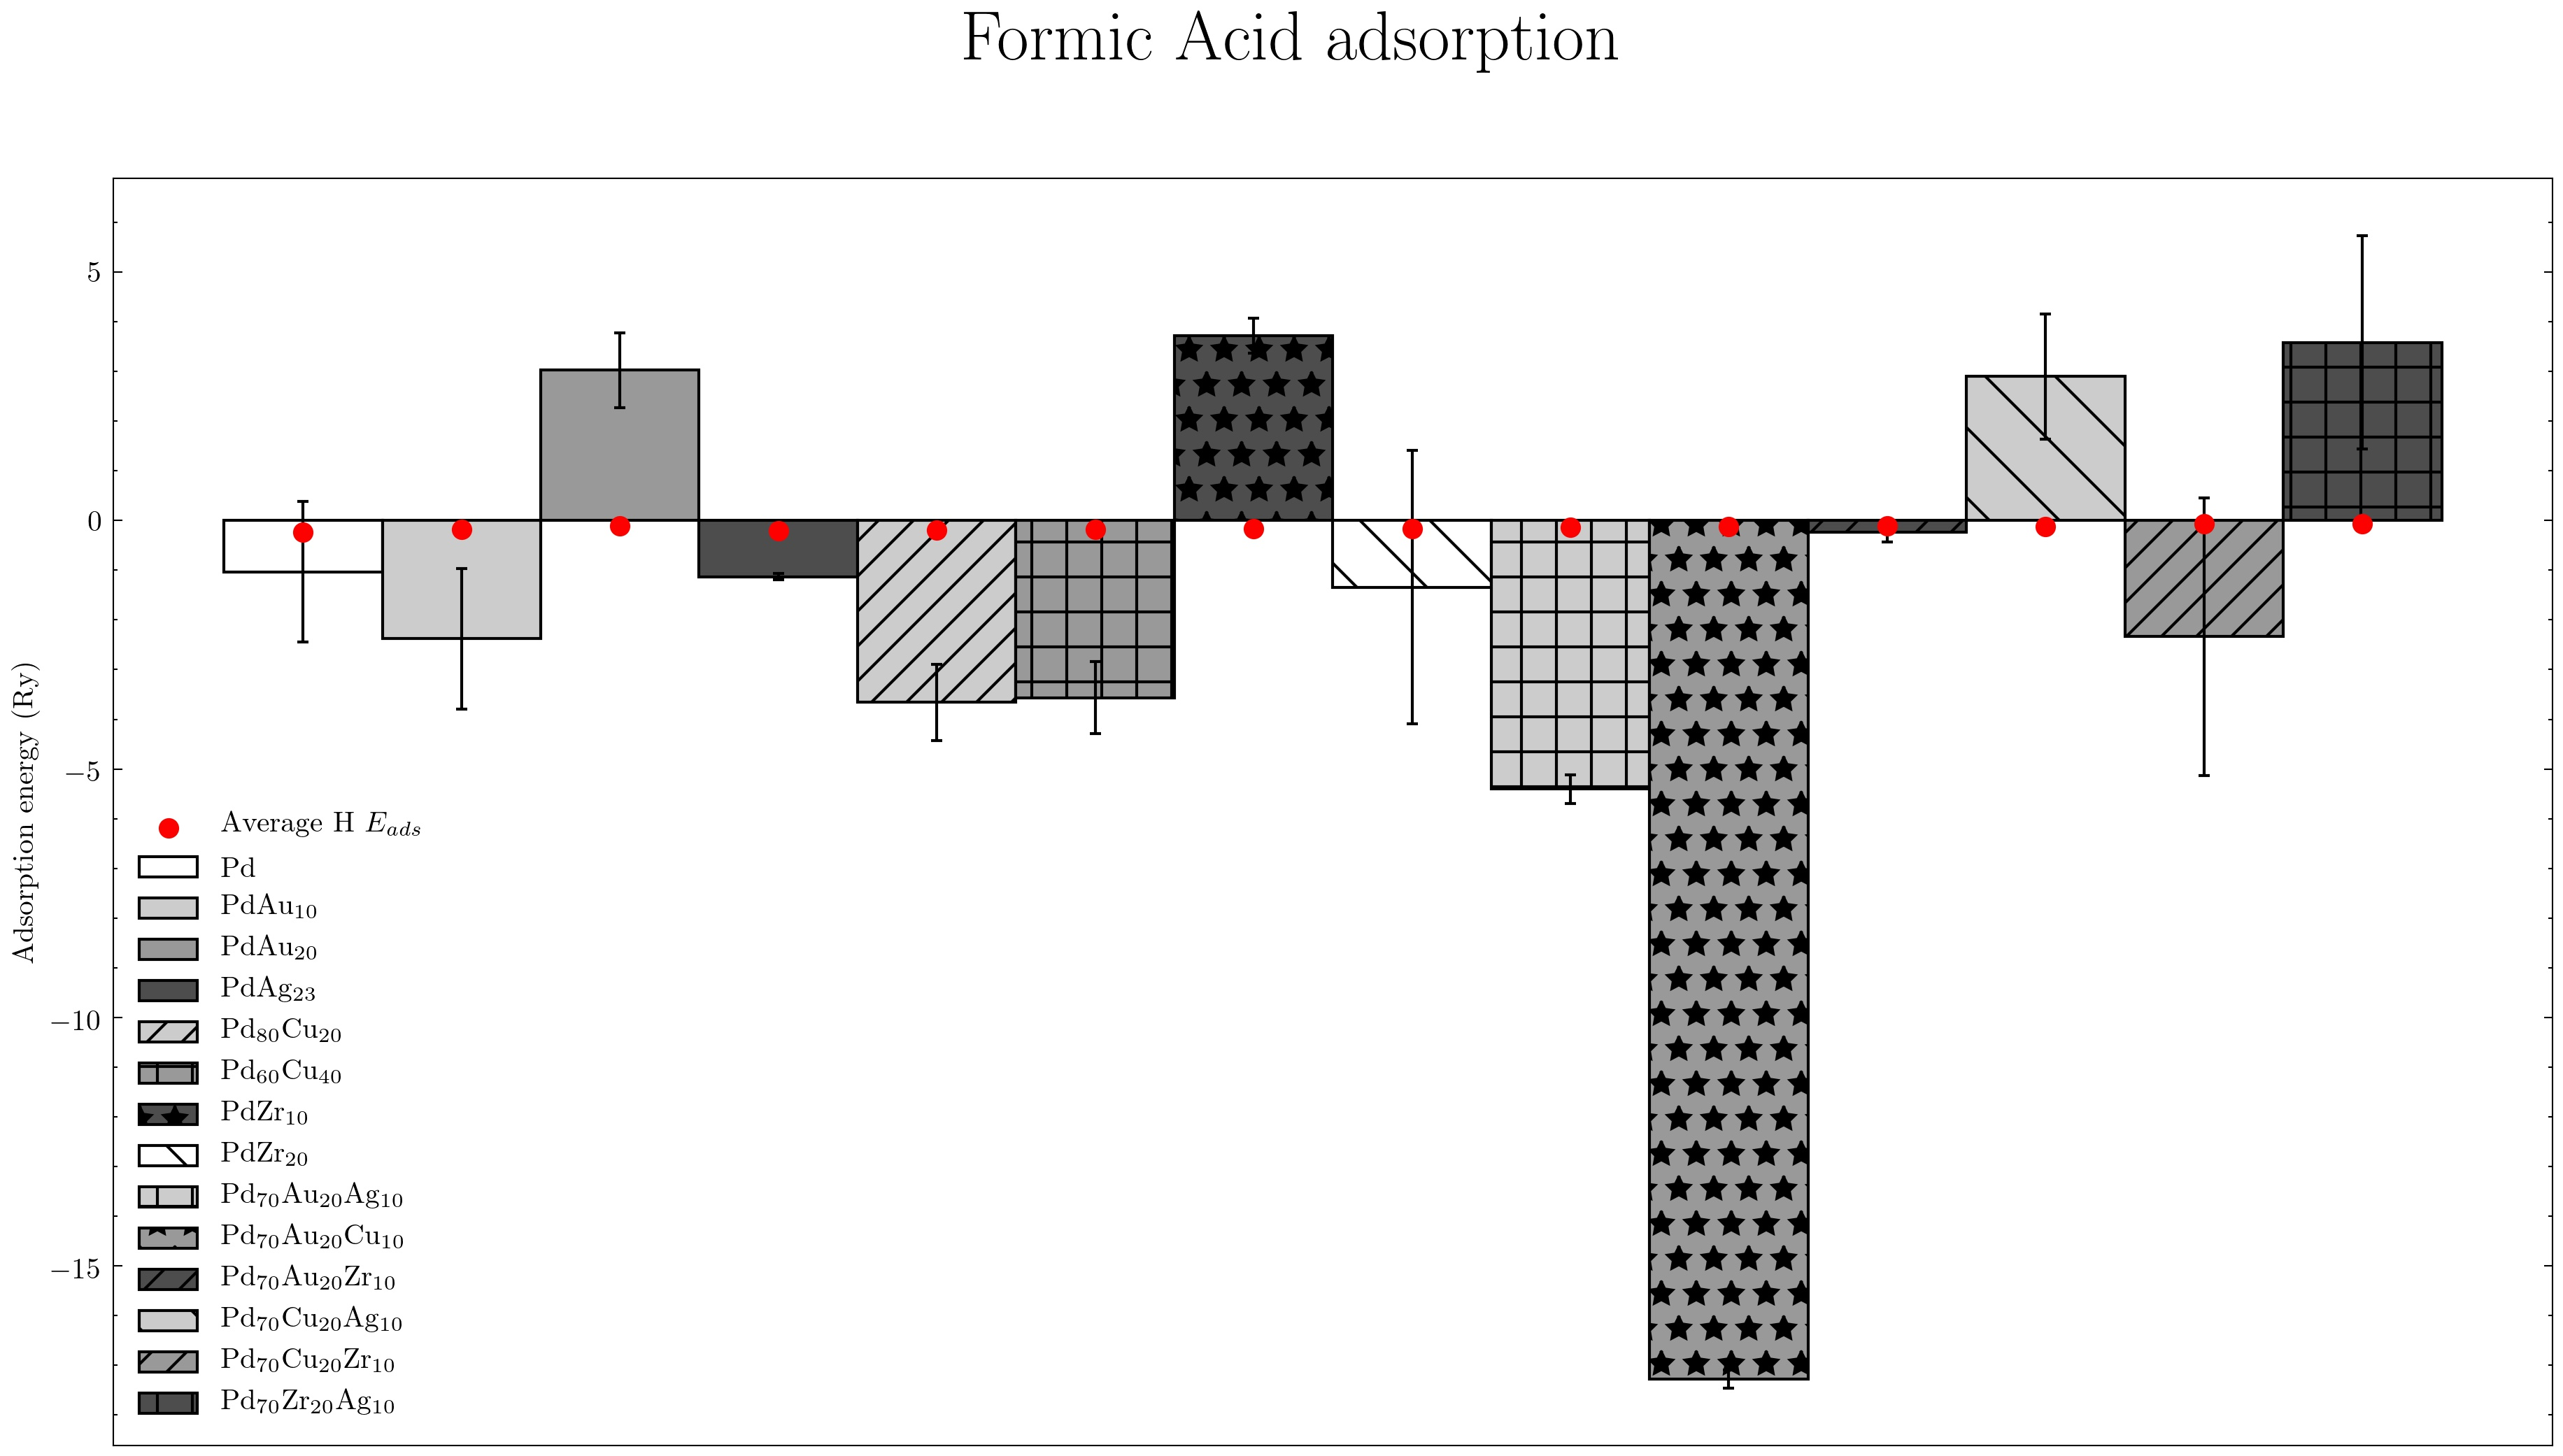
\includegraphics[width=0.9\linewidth,height=\textheight, keepaspectratio]{/Users/marc/Thesis/Chapter3/data/FAads.jpg}
      \caption{Average binding energy of Formic Acid on the surface of palladium and palladium alloy slabs}
      \label{FAads}
    \end{figure}
  
  \end{landscape}
\subsubsection{Hydrogen sulphide}
The final molecule that was simulated was H\textsubscript{2}S. This molecule was adsorbed using the sulphur atom as this is the known mechanism for H\textsubscript{2}S binding on a metallic surface. \cite{Morreale2007} The results are shown in figure \ref{h2sads}. As expected all metals showed the ability to bind with the sulphur atom at least as strongly as hydrogen. Additionally the S atom will bind stronger to all active sites for hydrogen dissociation as shown by figure \ref{H2Ssite}.

It appears that alloying with most metals will do little to halt the binding of sulphur, except for gold and Zr. Alloying with these metals brings the binding energy to a level where it is around equal to that of hydrogen, and is therefore more managable. Additionally while alloying with silver on it's own appears to infact increase the ability for sulphur to bind onto the surface, the effect is completely negated when gold is present. 

Of the alloys tested PdAu\textsubscript{20}, both Zr binary alloys, PdAuZr, PdCuAu, and PdZrCu appear to be the most suitable for mitigating the effects of H\textsubscript{2}S. It should be noted that past studies have revealed that Pd\textsubscript{4}S is in fact avaliable for hydrogen permeation, albeit at a much slower rate.\cite{Morreale2007} This may indicate that it is possible to pretreat a palladium membrane with sulphur, to a point where it is no longer reactive to sulphur, but can still permeate hydrogen. Such studies are outside the scope of this thesis however

\begin{figure}
  \centering
  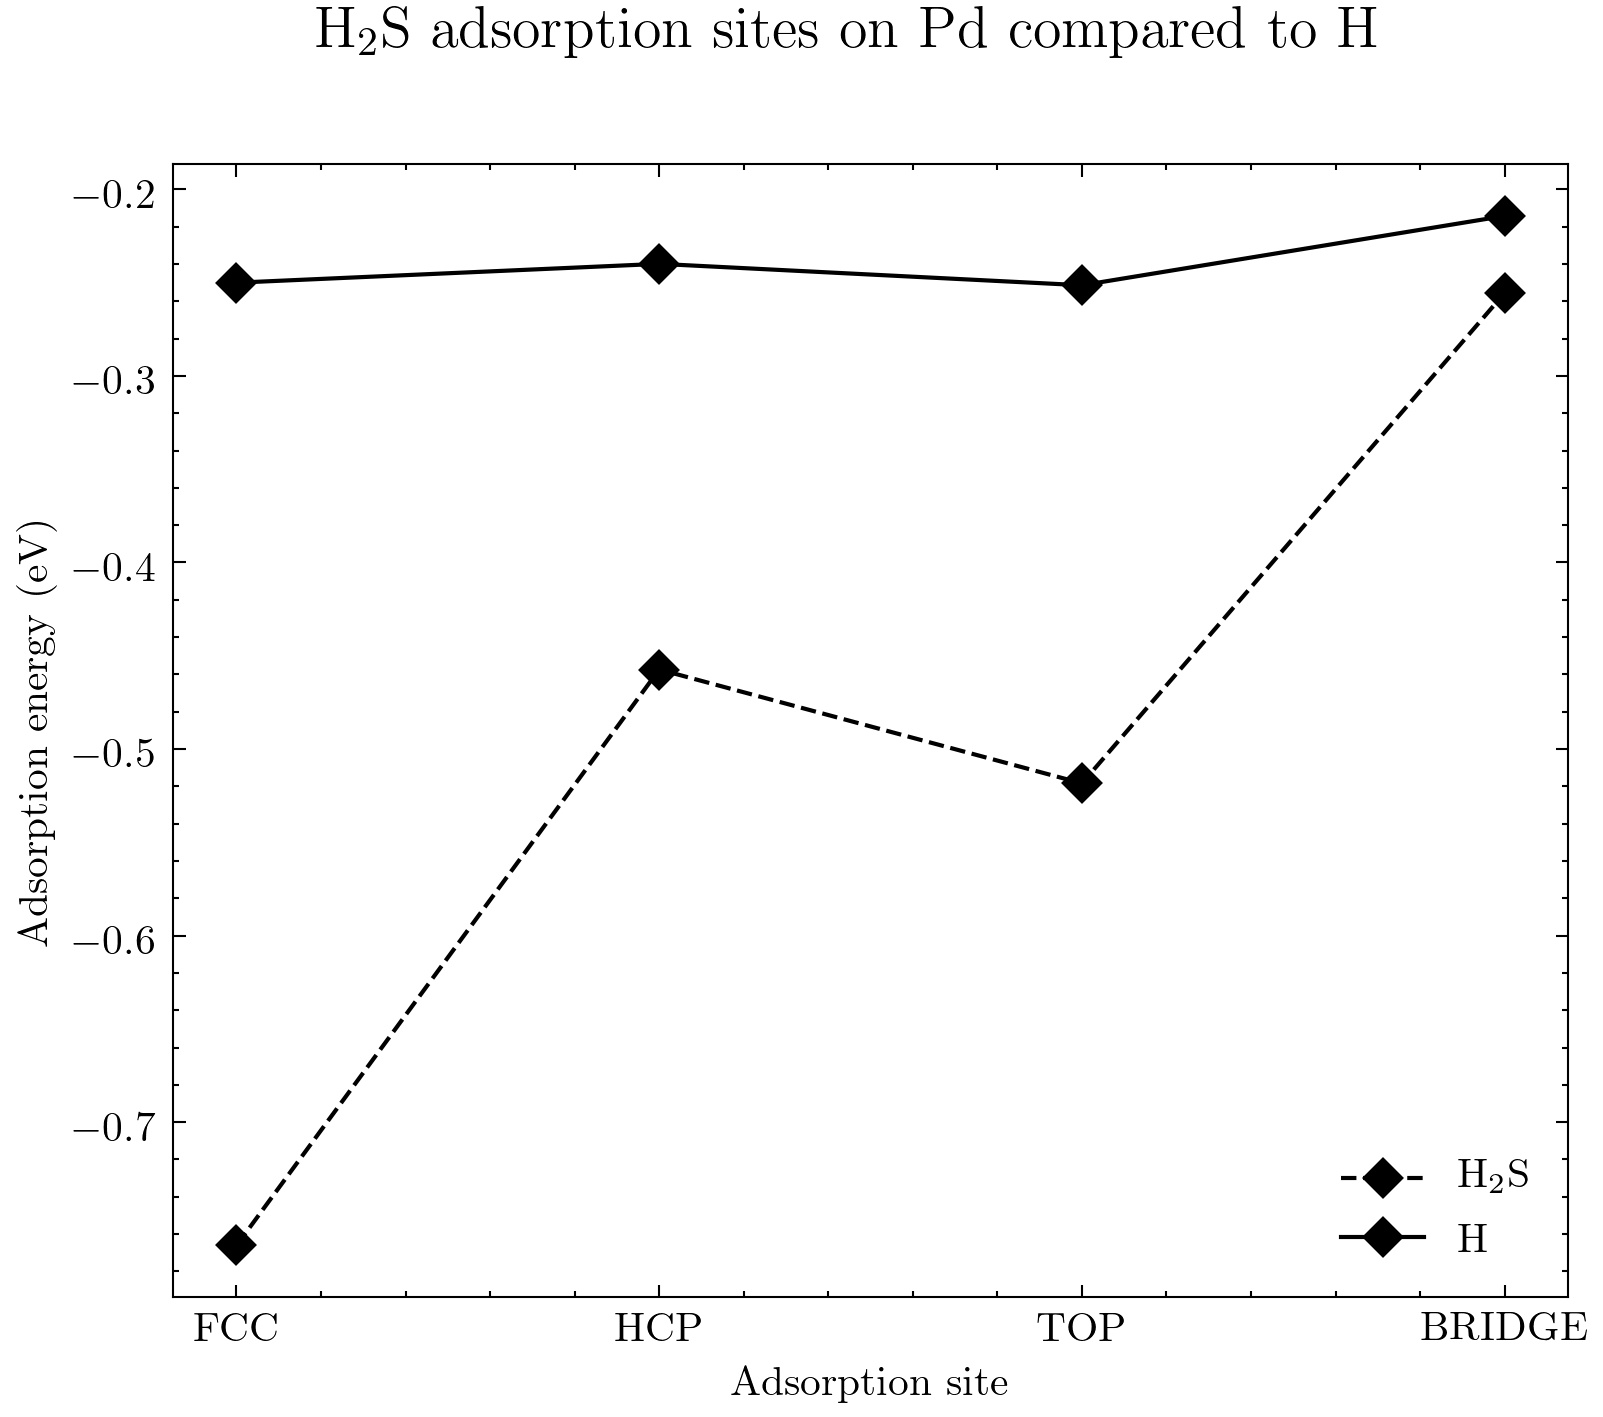
\includegraphics[width=0.7\linewidth, keepaspectratio]{/Users/marc/Thesis/Chapter3/data/H2SSites.jpg}
  \caption{binding energy of H and H\textsubscript{2}S for each site on a 2x2x5 Pd slab}
  \label{H2Ssite}
\end{figure}

\begin{landscape}

\begin{figure}
    \centering
    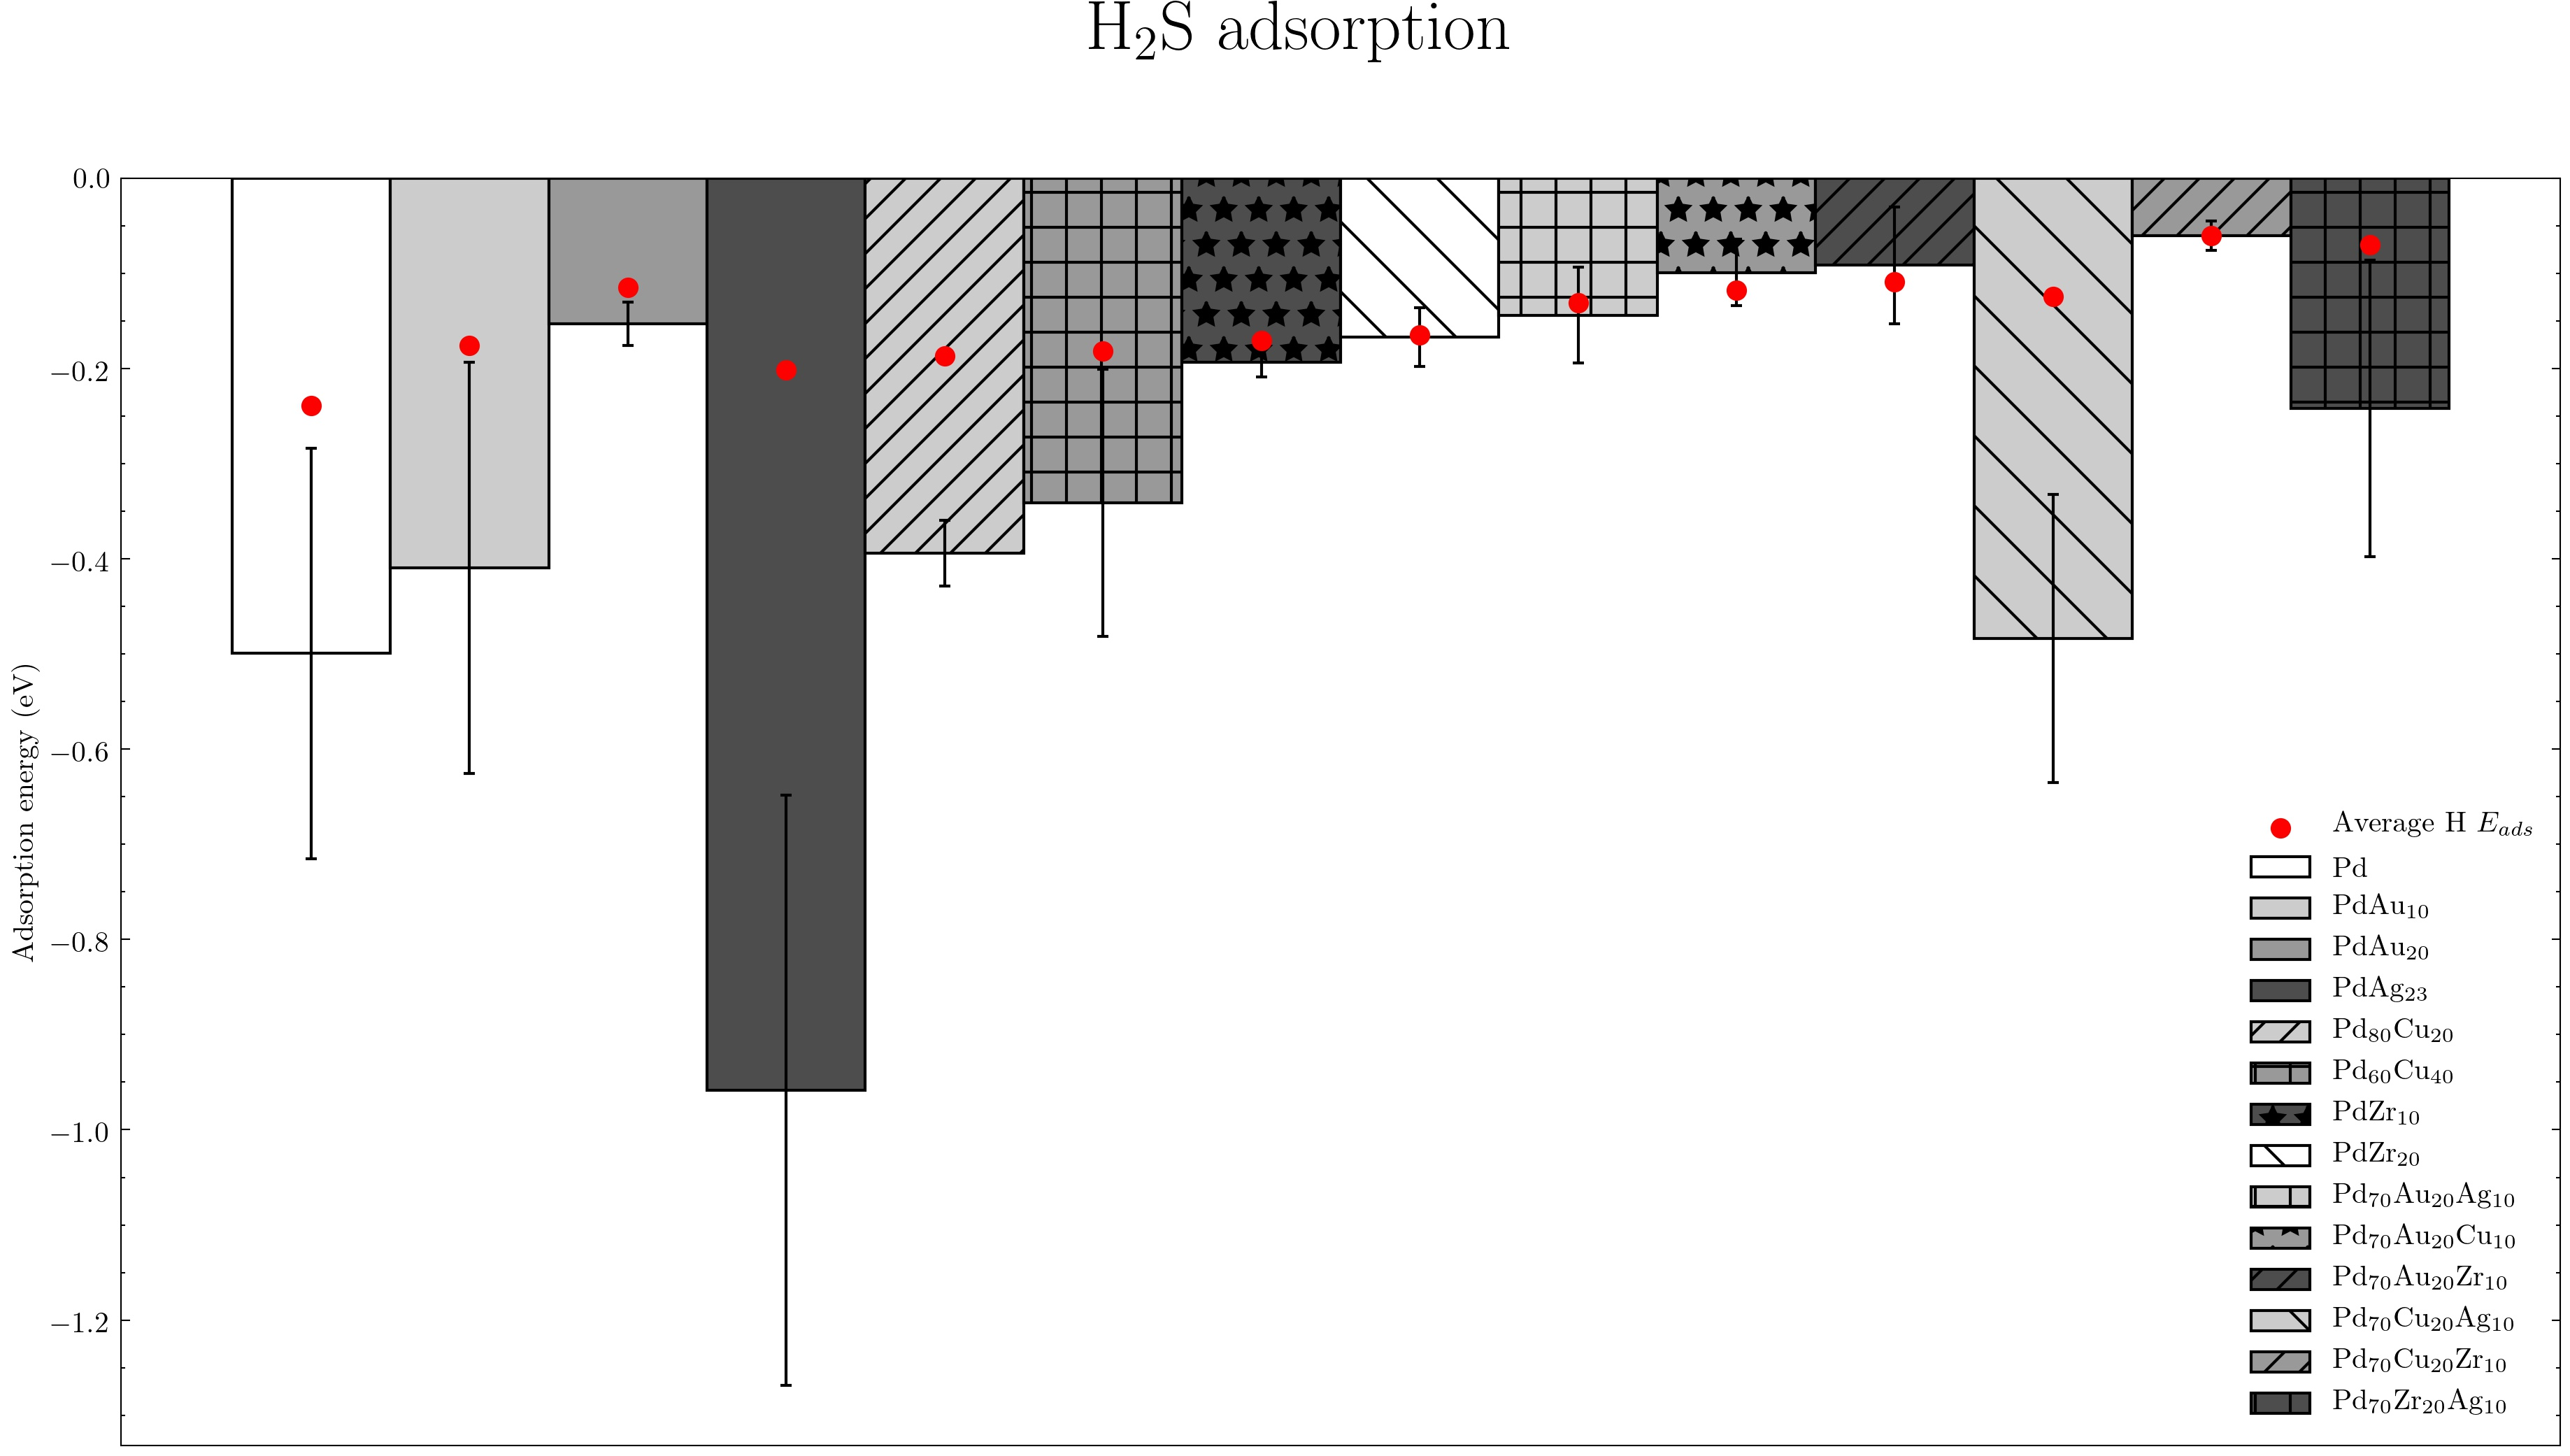
\includegraphics[width=0.9\linewidth,height=\textheight, keepaspectratio]{/Users/marc/Thesis/Chapter3/data/H2Sads.jpg}
    \caption{Average binding energy of H\textsubscript{2}S on the surface of palladium and palladium alloy slabs}
    \label{h2sads}
  \end{figure}
\end{landscape}


\section{Conclusion}
DFT simulations were carried out investigating the binding energies of ISO 14687-2 impurities on the surface of palladium and palladium alloy membranes. A number of metals were alloyed, either because they are commonly used in literature, or are known for their resistance to sulphur containing environments which were of key importance to this thesis. Most alloys were found to be stable except for Cr containing alloys, which were eliminated from the study. 

After testing the impurities it was clear that the binding of CO, CH\textsubscript{4}, O\textsubscript{2}, H\textsubscript{2}O and H\textsubscript{2}S were affected most by the alloy composition. Ar, He, N\textsubscript{2}, NH\textsubscript{3}, CO\textsubscript{2}, and Formic acid were found to be completely inert to all compositions. Formaldehyde strongly adsorbed to all alloys regardless of composition and further research will have to be taken to find a suitable composition to mitigate this. 

These impurities can be split into 3 broad groups, oxidising (O\textsubscript{2} and H\textsubscript{2}O) carbonaceous (CH\textsubscript{4} and CO) and sulphurous (H\textsubscript{2}). The best performing alloys for each of these impurities were decided by comparing the calculated binding energy to that of the same alloy binding with Hydrogen. The most suitable alloys for each class of material is shown in table \ref{finalresult}.

\begin{table}[]
  \centering
  \caption{Best performing alloys for each environment with respect to the different between the binding energies with relevant impurities, and the binding energy of hydrogen}
  \label{finalresult}
  \begin{tabular}{@{}ccc@{}}
  \toprule
  Environment  & Best performing alloy(s)                                & \begin{tabular}[c]{@{}c@{}}$E_{i_{ads}}/E_{H_{ads}}$ \\ \\ ($i$=impurity)\end{tabular}           \\ \midrule
  Oxidising    & PdAu20                                                  & -38.73 (H\textsubscript{2}O), -7.18 (O\textsubscript{2})                                                         \\
  Carbonaceous & \begin{tabular}[c]{@{}c@{}}PdAu\textsubscript{20}\\ PdAuCu\end{tabular} & \begin{tabular}[c]{@{}c@{}}0.50(CO) 0.40 (CH4)\\ 0.70(CO) 0.36(CH\textsubscript{4})\end{tabular} \\
  Sulphurous   & \begin{tabular}[c]{@{}c@{}}PdAuCu\\PdCuZr\\ PdAuZr\end{tabular} & \begin{tabular}[c]{@{}c@{}}0.84\\0.92\\ 0.98\end{tabular}                              \\ \bottomrule
  \end{tabular}
  \end{table}

In the following chapter these membreanes will be manufactured and tested under carbonaceous and sulphur containing environments in order to validate the results of this study. Oxygen containing environments will not be tested due to the dangers of heating oxygen in a hydrogen matrix.


\bibliographystyle{unsrtnat}
\bibliography{library.bib}